\documentclass[12pt,a4paper]{article}

\usepackage{amsmath}
\usepackage{physics}
\usepackage[utf8]{inputenc}
\usepackage{graphicx}
\usepackage[sorting=none]{biblatex}
\usepackage{float}
\usepackage{caption}
\usepackage{subcaption}
\usepackage{tikz}
\usepackage[separate-uncertainty=true]{siunitx}
%\usepackage{tikz-feynman}
\usepackage[hidelinks]{hyperref}

% TODO:
% 	- Omskrive Monte Carlo Måske?
%   - Discussion
%   - Conclusion
%   - Titlepage
%   - Update (maybe fix) fit to delphes data
% 	- Langtool


\addbibresource{References.bib}
\nocite{*}

\numberwithin{equation}{section}

\begin{document}

TITLE\\
AUTHORS\\
DATE

\cleardoublepage{}
\begin{abstract}
  This thesis studies the $Wtb$ vertex structure, using data ATLAS data from top
  quark decays, derived from $t\bar t$ events. The events are reconstructed with
  missing transverse momentum, single lepton decay and at least four jets where
  two of those jets are tagged as $b$ jets. The ATLAS Open Data, used in this
  thesis, was taken from $pp$ collisions at a centre-of-mass energy of $13$ TeV,
  which corresponds to a integrated luminosity of 10 $\mathrm{fb}^{-1}$. Angular
  asymmetries is used as the primary method for measuring the polarisation of
  the $W$ bosons, with a secondary approach of fitting Delphes $W$ polarisation
  simulations to data taken from the ATLAS detector. The measured helicity
  fractions from Angular asymmetries are $F_0=0.678 \pm 0.015$,
  $F_L=0.308 \pm 0.008$ and $F_R=0.014 \pm 0.009$, with only statistical
  uncertainties considered, and angular asymmetries of $A_+ = 0.542 \pm 0.005$
  and $A_- = -0.831 \pm 0.007$, in agreement with the Standard Model.

\end{abstract}
\cleardoublepage{}
\tableofcontents{}
\cleardoublepage{}
\section{Introduction}
The standard model (SM) of particle physics is very successful at describing the
fundamental constituents of matter in our universe. Through experiments with
particle accelerators, many of the theoretical details in the SM has been
corroborated. To further test the theory larger accelerators are needed, which
led to the construction of the large hadron collider (LHC), finished in 2008.
Particles are collided together at high energy to probe the properties of the
produced debris, hoping to discover new physics that deviates from the SM.\\

The top quark was discovered in 1995, by experiments done by CDF~\cite{Abe_1995}
and DØ~\cite{Abachi_1995}. It is the heaviest known fundamental particle, with a
mass of $172.76 \pm 0.30 \mathrm{GeV/c^2}$~\cite{pdg}, and its coupling
strength to all the bosons are well predicted by the standard model. Because of
its heavy mass and consequently short lifetime, it doesn't have enough time to
bind with lighter quarks and form hadrons before it decays, which means that it
effectively decays, to a good approximation, as a free quark. Measurements of
the top quark's properties plays an important role in testing the Standard
Model. Top quark production at LHC occurs via strong interactions, where they
are produced in top, anti-top pairs. One test of the Standard Model, is the
study of the $Wtb$ vertex Lorentz structure and coupling, which is studied by
looking at the decay products of top quarks. The top quarks decay, with almost
100\% branching fraction, by weak interactions into $W$ bosons and bottom quarks
$t \rightarrow W + b$. The $W$ bosons decay, into either a charged lepton and neutrino;
$W \rightarrow l + \nu_l$, or into a quark, anti-quark pair: $W \rightarrow q' + \bar{q}$, as
illustrated in the Feynman diagram Figure~\ref{fig:feynmandiagram}.\\

\begin{figure}[H]
	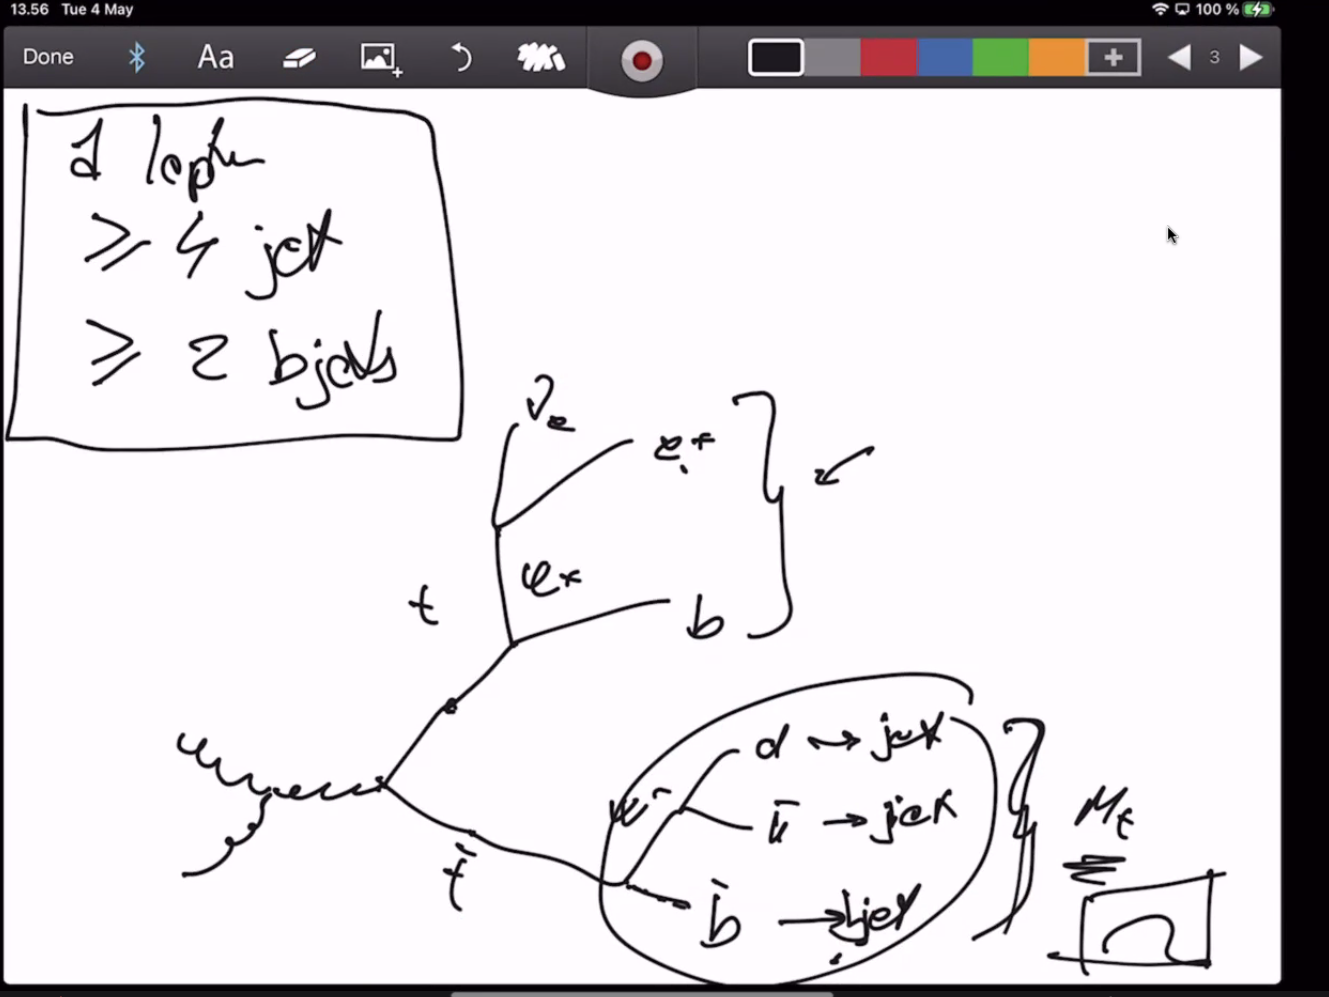
\includegraphics[width=\linewidth]{figures/placeholder_feynman_singlelep.png}
  %\begin{center}
  %  \feynmandiagram[horizontal=a to start, tree layout] {
  %    a     -- [gluon] start -- [fermion, edge label=$t$] t,
  %    t     -- [boson, edge label=$W^+$] Wp,
  %    Wp    -- [fermion] v [particle=$\nu_e$],
  %    Wp    -- [anti fermion] e [particle=$e^+$],
  %    t     -- [fermion] b [particle=$b$],
  %    start -- [anti fermion,edge label'=\(\overline{t}\)] tbar,
  %    tbar  -- [boson, edge label=$W^-$] Wm,
  %    Wm    -- [fermion] d [particle=$d$],
  %    Wm    -- [anti fermion] u [particle=$\overline{u}$],
  %    tbar  -- [anti fermion] bbar [particle=$\overline{b}$],
  %    };
  %\end{center}
	\caption{The Feynman diagram shows the chain of decay, that results in single
    leptonic decay, for pair $t\bar t$. The diagram illustrates the final
    product of the reaction; at least four jets and a lepton neutrino
    pair.}\label{fig:feynmandiagram}
\end{figure}

In this report, we are only looking at decays with a single lepton as decay
product. The leptons we look at are either electrons or muons, and the collision
will produce four jets, as evident from the diagram.

\section{Theory}

\subsection{Standard Model}
The Standard Model is a relativistic quantum field theory that describes three
of the four fundamental forces, (the electromagnetic force, the strong force and
the weak force), into a single theoretical framework. It contains all the known
elementary particles, and how these particles interact with the different
fields. The standard model manages to unify the electromagnetic (EM), and the
weak force into different aspects of the same force called the electroweak
force, while describing strong interactions through the framework of Quantum
Chromodynamics.\\

The elementary particles can be split into two distinct categories, called
fermions and bosons. Fermions are defined by their spin, which is a half integer
spin, and is exclusively $1/2$ for all the elementary fermions of the Standard
Model. They obey the Pauli exclusion principle which means that two identical
fermions can't occupy the same quantum state. The fermions are grouped into
quarks and leptons, each with three generations or families based on their
masses. All the fermions have an antiparticle associated with them, each with
opposite charge, and apart from these antiparticle partners, there are a total
of twelve known fermions, two leptons and two quarks in each family. The quarks
that pair together in each generation are; the up and down quark, the charm and
strange quark, and the top and bottom quark. The leptons, electron, muon and
tau, each pair together with a neutrally charged neutrino.\\

%evt. insætte billede om SM tabellen her.

In the SM, the fermions interact via gauge bosons, integer spin particles, which
include the photon, gluon, $W$- and $Z$-boson, also called force carrier
particles of the: electromagnetic force, the strong force and the weak force
respectively. Quarks interact with the EM and the strong force, while leptons
interact only with the electroweak force. Because neutrinos are neutrally
charged, they will only interact via the weak force. Several unique features is
found in weak interactions, such as parity violation (P), violation of charge
conjugation (C), as well as a violation of the combined charge conjugation and
parity symmetry (CP). Weak interactions do obey the combination of charge
conjugation, parity, and time reversal symmetry.

\subsubsection{Quantum Chromodynamics}
Quantum chromodynamics (QCD), is the theory of the strong interaction, which
binds the quarks together. In the year 1964, physicist Murray Gell-Mann and his
PhD student George Zweig, proposed that baryons and mesons could be explained by
the existence of smaller triplet particles\cite{GELLMANN1964214}. Since the
Pauli exclusion principle forbids any fermions from inhabiting the same state,
leading to the development of the concept of colour in 1973\cite{FRITZSCH1973365}
by physicists Harald Fritzsh, Heinrich Leutwyler and Murray Gell-mann,
suggesting that these quarks had additional conserved
quantum numbers, later named colour charge.\\

In QCD, each quark is associated with a colour charge that confines the quark via
the strong interaction to other quarks to make up a total colour charge that is
neutral. While the colour charge isn't physically related to actual colours, the
way they mix together, is analogous to the way we mix the colours green, red and
blue, as well as their anti colours, magenta, yellow and cyan. Because of these
properties, quarks can bind together in groups of three to form baryons, or in
groups of two to form mesons.\\

If enough energy is added to stretch one of the quarks away from the rest, the
gluon field breaks, and a new quark and anti quark pair is created. This process
of creating new quark, anti quark pairs, by stretching the gluon field between
them is the result of violent inelastic collisions, which creates these jets of
quarks, anti quarks.\\

\subsubsection{Symmetries and Laws of Conservation}
In the year 1918, Emmy Noether showed that any conservation law is associated
with a continues symmetry of the Lagrangian\cite{Noether_1971}. The
conservation laws of classical physics are the result of them being invariant
with respect to their canonically conjugate quantities. The conservation of
energy, linear momentum and angular momentum, stems from their invariance in
time, space and angles respectively. This implies that the laws of physics are
independent of the time, the location and the orientation in space.\\

Another symmetry, that is very important for quantum mechanics, is the
reflection symmetry, called parity. A wave function can have positive or
negative parity depending on whether or not it changes sign under parity
transformation. For the laws which are invariant under reflection in space, the
parity quantum number $P$ is conserved, while in relativistic quantum mechanic,
we need to ascribe an intrinsic parity to particles and antiparticles.\\

Group theory gives the tools to study these symmetries more elegantly, and has
become particularly useful to describe symmetries of quantum mechanics, where
degenerate eigenstates furnishes irreducible representations of a group. In
studying these groups, we can discover other conserved quantities in the
interactions of the EM, the weak or the strong force.\\

The Gauge invariance of the unitary group U(1), leads to conservation of
electric charge, as well as the conservation of lepton number. Lepton number
conservation is, far as we know, conserved in all interactions. Certain
particles behave practically identically with respect to the strong or the weak
interactions, these properties are studied through irreducible representations
of the group SU(3), and are characterized by strong and weak isospin, which are
also conserved.\\

The Dirac equation extends the Schrödinger wave equations, to include the
effects of special relativity. The solution to this equation shows that for
relativistic particles, where $\beta = v/c \rightarrow 1$, the projection of a particle's spin
onto the direction of their momentum is conserved. This conserved quantity is
called helicity\cite[63]{Povh2015} and is defined as
\begin{equation}
  h = \frac{\vb{s \cdot p}}{\abs{\vb s} \cdot \abs{\vb p}},
\end{equation}
where $\vb s$ is the spin, and $\vb p$ is the momentum of the particle. For
spin 1 particles, the Gauge bosons, the particle can take on three distinct
helicity values, $h=-1$, $h=0$ and $h=1$, which corresponds to left-handed,
longitudinal and right-handed respectively.\\

Chirality is a fundamental property of a particle determined by representation
theory. In the relativistic limit the distinction between helicity and chirality
disappears, as the mass term $mc^2$ becomes negligible compared to the total
energy. The weak force will only interact with left-chiral particles and
right-chiral antiparticles. The operator of an interaction that describes the
exchange of a boson, can have both vector $V$ and axial vector $A$ nature. If it
has both a vector and an axial part, as in the case of weak interactions, parity
is violated, and maximum parity violation occurs when both the contributions
becomes equal magnitude, which is true for (V-A) structures..\\

After the discovery of parity violation and charge conjugation, in weak
interactions, by physicist C.S Wu\cite{PhysRev.105.1413}, it was believed by
physicists that CP-symmetry, the combination of charge conjugation symmetry and
parity, was a true symmetry of the Standard model, until that too was violated
in weak decay of neutral kaons, forcing physicists to reformulate the
electroweak interaction in the Standard Model. The Cabbibo-Kobayashi-Maskawa
(CKM) matrix explains how the flavour eigenstates of the quarks are related to
the mass eigenstates, and is a $3 \times 3$ unitary matrix, with four independent
parameters: three real angles and an imaginary phase\cite[153]{Povh2015}. The
imaginary phase gives rise to CP violation, but the matrix preserves CPT
symmetry.

\subsection{Momentum}\label{sec:momentum}

\subsubsection{Four-momentum}
The data collected in LHC collisions, allows us to reconstruct the four-vector
of momentum for the involved particles, the Lorentzvector. This four-vector is a
four component tensor, made up of an ordinary three-dimensional vector for
relativistic momentum $\vb p$, and the relativistic energy term, $E/c$, as its
zeroth component. Working in natural units, where $c=1$, the four-vector will be
given as
\begin{equation}
p = \left(\begin{matrix} E \\ \vb p \end{matrix} \right).
\end{equation}

The dot product of two four-vectors is defined for this Lorentzvector as;
$p\cdot p' = E E' - \vb p \cdot \vb{p'}$, where $\vb p \cdot \vb{p'}$ is the ordinary dot
product of two three-dimensional momentum vectors. From special relativity, it is known
that $E^2 - \abs{\vb p}^2 = m^2$, so from the four-vector dot product of two
identical four-vectors, the following holds true $p^2 = m^2$. Other vector
operations on a four-vector is similar to the same vector operations on a
three-dimensional vector. The quantity
\begin{equation}
s = (p + p')^2 = (E + E')^2 - (\vb p + \vb p')^2
\end{equation}
is a conserved quantity, the centre-of-mass energy squared of the system. It is
the square of the collision energy, which allows the creation of new particles,
and allows the probing of particles' properties.

\subsubsection{Transverse Momentum}\label{sec:transmomentum}
In LHC experiments, the protons gets smashed together in head-on collisions at
nearly the speed of light. Since the protons momenta are parallel to the beam
axis, conventionally defined as the $z$-axis, their total momentum in the
$xy$-plane, the transverse momentum $\vb p_T$, is zero. The jets scatter off in
new directions, at angles given by the polar angle $\theta$, and the azimuthal angle
$\varphi$. The polar angle is defined as the angle of the jet, with respect to the
$z$-axis, while the azimuthal angle is defined as the angle of the jet, with
respect to the $x$-axis in the $xy$-plane, as seen in Figure~\ref{fig:momentum}.

\begin{figure}[H]
  \centering
  % 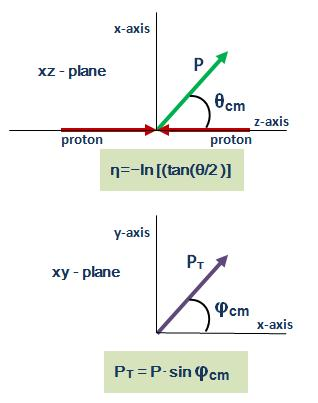
\includegraphics{figures/momentum.jpg}
  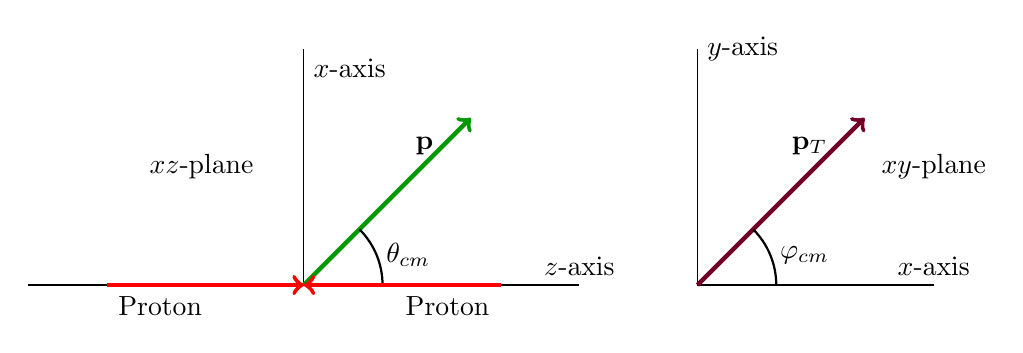
\begin{tikzpicture}
    \draw (-3.5, 0)--(3.5, 0) node[anchor=south] {$z$-axis};
    \draw (0,0) --(0,3) node[anchor=north west] {$x$-axis};
    \draw[green!60!black, ->, ultra thick]  (0, 0) -- (45:3);
    \draw[thick] (1,0) arc (0:45:1);
    \draw (45:2.5) node[anchor=east,black] {$\vb p$};
    \draw (22.5:1) node[anchor=west] {$\theta_{cm}$} ;
    \draw[ultra thick, red, <-] (0,0) -- (2.5,0) node [anchor=north east, black] {Proton};
    \draw[ultra thick, red, <-] (0,0) -- (-2.5,0) node [anchor=north west, black] {Proton};
    \draw (-1.3, 1.5) node {$xz$-plane};

    \draw (8,0) node [anchor=south] {$x$-axis} -- (5,0) -- (5,3) node [anchor=west] {$y$-axis};
    \draw[purple!60!black, ->, ultra thick]  (5, 0) -- +(45:3);
    \draw[thick] (6,0) arc (0:45:1);
    \draw (5,0)+(22.5:1) node[anchor=west] {$\varphi_{cm}$} ;
    \draw (5,0)+(45:2.5) node[anchor=east,black] {$\vb p_T$};
    \draw (8,1.5) node {$xy$-plane};
  \end{tikzpicture}
  \caption{The figure shows the momentum traveling parallel to the beam axis, and
  the transverse momentum, each with their respective angles.\label{fig:momentum}}
\end{figure}

In cylindrical detectors, it is useful to use another magnitude called
pseudorapidity, which ranges from values between $(-\infty, \infty)$. Pseudorapidity is
related to the polar angle, and is defined as:

\begin{align}
\label{eq:pseudorapidity}
\eta = -\ln({\tan\left(\frac{\theta}{2}\right)}).
\end{align}

In particle collisions, the longitudinal momenta of the colliding elementary
gluons and quarks are unknown. These carry an unknown amount of the protons'
momenta, where the remaining momentum disappears into the beam tube. To
reconstruct the jets' tracks, the transverse momentum is analysed, but not all
particles are detected by ATLAS, such as the small neutrally charged neutrinos,
their existence is understood by the conservation of momentum. The missing
transverse momentum $E_T^{miss}$ is defined as the transverse momentum that is
not detected by the detector, but calculated as the momentum for which the total
momentum of the system will add to zero~\cite{xabier}.

\subsection{Top Quarks}
The top quark is the third generation up-type quark in the SM, with a charge of
$+2/3 e$, and the greatest mass of all the known elementary particles. Top quark
has a weak two-body decay and its decay can be analysed from the
Cabbibo-Kaboyashi-Maskawa matrix (CKM). The diagonal part of the CKM matrix,
shows quarks transition predominantly within their own family, with very little
deviation from unity. This is especially true for the top quark, where top
quarks decays into bottom quarks and $W$ bosons 99.8\% of the time. Because the
top quark decays as a free quark, we can use the polarisation as an observable,
because its spin will be preserved in the decay product.\\

There are two primary mechanisms for the production of top quarks at the LHC, a
single top via weak interactions, or the pair production via the strong force.
The pair production of top quark is a QCD effect, which takes place by gluon
fusion $gg \rightarrow t\bar t$ and quark-antiquark annihilation $q\bar q \rightarrow t\bar t$. The
branching fraction of each of the pair production processes, is related to the
centre-of-mass energy, for which gluon fusion dominates at the LHC at about 86\%
of the production\cite{dasilva2016quark}.
\begin{figure}[H]
  \centering
	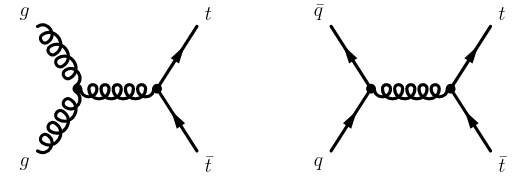
\includegraphics[width=\linewidth]{figures/placeholder_feynman_ttproduction.png}\\
  %\hfill{}
  %\feynmandiagram[layered layout,horizontal=a to b] {
  %  g1 [particle=$g$] -- [gluon] a [dot],
  %  g2 [particle=$g$] -- [gluon] a,
  %  a  -- [gluon] b[dot],
  %  b  -- [fermion] t [particle=$t$],
  %  b  -- [anti fermion] tbar [particle=$\overline{t}$],
  %};\hfill{}
  %\feynmandiagram[layered layout,horizontal=a to b] {
  %  qbar [particle=$\overline{q}$] -- [anti fermion] a [dot],
  %  q [particle=$q$] -- [fermion] a,
  %  a  -- [gluon] b[dot],
  %  b  -- [fermion] t [particle=$t$],
  %  b  -- [anti fermion] tbar [particle=$\overline{t}$],
  %};
  %\hfill{}
	\caption{A Feynman diagram of the two main production processes $gg \rightarrow t\bar t$
    on the left, and $q\bar q \rightarrow t\bar t$ on the right. Both produciton
    mechanisms are results of strong interactions.}\label{fig:ttproduction}
\end{figure}

\subsection{Coupling of W$^+$tb}\label{sec:coupling}
The leptonic decay of the $W$-boson, can decay into either of the three leptonic
families, with nearly equal branching ratios. The $\tau$ lepton is also very
unstable and has too short a lifetime, so it does not get tagged in this thesis.
$\tau$-particles that decay by weak interaction into electrons,
$\tau^+ \rightarrow e^+ \nu_e \bar \nu_{\tau}$, or muons, $\tau^+ \rightarrow \mu^+ \nu_\mu \bar \nu_{\tau}$, are tagged as part of
the single lepton channel.\\

The $W$-boson couples only to left-handed fermions, or right-handed
anti-fermions, giving $Wtb$ vortex a (V-A) structure. In the Standard Model we
expect that the $W$-boson and $b$-quark from top decay, arrange such that chiral
structure of the coupled vertex is fulfilled. Because of parity violation, the
events with positive helicity (right polarised) gets suppressed, while events
with negative (left polarised) and longitudinal helicity dominates. The three
polarisations are illustrated in Figure~\ref{fig:polarisation}, where, in this
hyper relativistic limit the $b$ quark can, to a good approximaiton,
$m_t >> m_b$, always be considered left handed, which necessitates that the $W$
boson is either longitudinal or right handed.

\begin{figure}[H]
  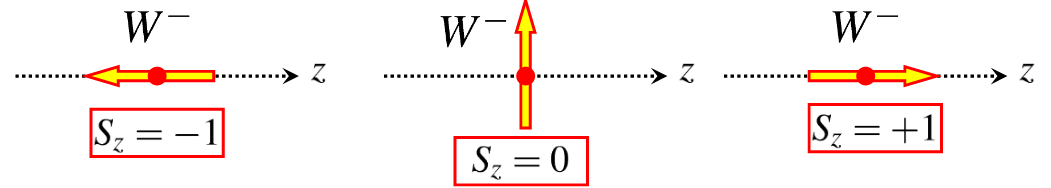
\includegraphics[width=\linewidth]{figures/w_polarization.png}
  \begin{tikzpicture}
    %\draw[dashed, ->] (-6.6,0) -- (-2.4,0);
    %\draw[-latex, line width=2,red] (-4.8,0) -- (-4,0);
    %\draw[-latex, line width=2,red] (-3.3,0) -- (-2.5,0);
    %\draw[-latex, line width=2,red] (-6,-0.3) -- (-6,0.4);
    %\draw[-latex, line width=3,teal!80!white] (-6.4,0.7) -- (-5.3,0.7);
    %\draw[-latex, line width=3,yellow!95!black] (-2.5,0.7) -- (-3.6,0.7);
    %\filldraw[black] (-4.5,0) circle (0.05) node[anchor=north,black] {$t$};
    %\filldraw[black] (-3,0) circle (0.05) node[anchor=north,black] {$b$};
    %\filldraw[black] (-6,0) circle (0.05) node[anchor=north west,black] {$W$};
    %\draw (-4.5,1.5) node[anchor=south] {Longitudinal(0)};
    %\draw (-4.5,-0.5) node[anchor=north] {\Large $h_W=0$};
    %
    %\draw[dashed, ->] (-2.1,0) -- (2.1,0);
    %\draw[-latex, line width=2,red] (-0.3,0) -- (0.5,0);
    %\draw[-latex, line width=2,red] (1.8,0) -- (1,0);
    %\draw[-latex, line width=2,red] (-1.8,0) -- (-1,0);
    %\draw[-latex, line width=3,teal!80!white] (-1,0.7) -- (-2.1,0.7);
    %\draw[-latex, line width=3,yellow!95!black] (1,0.7) -- (2.1,0.7);
    %\filldraw[black] (0,0) circle (0.05) node[anchor=north,black] {$t$};
    %\filldraw[black] (1.5,0) circle (0.05) node[anchor=north,black] {$b$};
    %\filldraw[black] (-1.5,0) circle (0.05) node[anchor=north,black] {$W$};
    %\draw (0,1.5) node[anchor=south] {Left-handed(L)};
    %\draw (0,-0.5) node[anchor=north] {\Large $h_W=-1$};
    %
    %\draw[dashed, ->] (2.4,0) -- (6.6,0);
    %\draw[-latex, line width=2,red] (4.2,0) -- (5,0);
    %\draw[-latex, line width=2,red] (2.7,0) -- (3.5,0);
    %\draw[-latex, line width=2,red] (6.3,0) -- (5.5,0);
    %\draw[-latex, line width=3,teal!80!white] (2.6,0.7) -- (3.7,0.7);
    %\draw[-latex, line width=3,yellow!95!black] (6.4,0.7) -- (5.3,0.7);
    %\filldraw[black] (4.5,0) circle (0.05) node[anchor=north,black] {$t$};
    %\filldraw[black] (3,0) circle (0.05) node[anchor=north,black] {$b$};
    %\filldraw[black] (6,0) circle (0.05) node[anchor=north,black] {$W$};
    %\draw (4.5,1.5) node[anchor=south] {Right-handed(R)};
    %\draw (4.5,-0.5) node[anchor=north] {\Large $h_W=+1$};
  \end{tikzpicture}
  \caption{The figure illustrates W-boson with zero, negative and positive
    helicity, corresponding to a longitudinal, left and right handed
    polarisation. The red arrows indicates the momentum direction of the
    particles, while the teal and yellow arrows indicate the spin orientation.
    The right handed polarisation will be heavily suppressed because of the
    (V-A) structure of the Wtb vertex.}\label{fig:polarisation}
\end{figure}

The fraction of; longitudinally $F_0$, left $F_L$ or right $F_R$ polarised
$W$-bosons which are produced from top quark decay, is referred to as helicity
fractions. In the Standard Model these fractions are calculated using quantum
chromodynamics. In leading order calculations, using the $m_b = 0$ limit, the
fractions are determined by the folllowing relations; $F_0/F_L = (m_t/m_W)^2$
and $F_R = 0 \Rightarrow F_0 + F_L = 1$, corresponding to the helicity fractions;

\begin{align}
\label{eq:helfrac}
  F_0 &= \frac{m_t^2}{m_t^2 + 2 m_W^2} \approx 0.7\\
  F_L &= \frac{2 m_W^2}{m_t^2 + 2 m_W^2} \approx 0.3\\
  F_R &= 0
\end{align}

For further corrections, these fractions are found in next to next to leading
order (NNLO) calculations to be $F_0 = 0.687 \pm 0.005$, $F_L = 0.311 \pm 0.005$
and $F_R = 0.0017 \pm 0.0001$\cite{Czarnecki_2010}. The experimental method to
extract these fractions is by studying the angular decay distribution of the
leptonic decay products of the top quark. The angular distribution is given by:

\begin{equation}
  \frac{1}{\Gamma}\dv{\Gamma}{\cos \theta^*} = \frac{3}{8}(1-\cos \theta^*)^2 F_L +
  \frac{3}{4}\sin^2 \theta^* F_0 + \frac{3}{8}(1+\cos \theta^*)^2 F_R.
\end{equation}

Where $\theta^*$ is the helicity angle, which is defined as the angle between the
charged lepton momentum direction, and the reversed momentum direction of the
decayed $b$ quark, viewed from a reference frame with $W$ at
rest~\cite{PhysRevD.45.124}. An expression for $\cos \theta^*$ can be found, using
the dot product of the two four-momentum vectors, the lepton $p_l$ and $b$ quark
$p_b$; $p_l\cdot p_b=E_bE_l-\vb{p_l\cdot p_b}=E_bE_l+\abs{\vb{p_l}}\abs{\vb{p_b}}\cos \theta^*$,
where the $\cos{(\theta^{*}-\pi)}=-\cos \theta^{*}$ was used to flip the sign.
$\cos \theta^{*}$ is then given by;


\begin{equation}
  \cos \theta^*=\frac{p_l\cdot p_b-E_lE_b}{\abs{\vb{p_l}}\abs{\vb{p_b}}}\\
  \simeq -\frac{p_l\cdot p_b}{E_lE_b} - 1 = \frac{2 M_{lb}^2}{m_t^2 - M_W^2} - 1. \label{eq:costheta}
\end{equation}
Where $M_{lb}$ is the invariant mass of the lepton and bottom quark system. The
approximation arises from the relativistic assumption that the masses of the
lepton and $b$ quark can be neglected so that
$E_lE_b\simeq \abs{\vb{p_l}}\abs{\vb{p_b}}$. The dependence is shown in
Figure~\ref{fig:distributions} for the three distribution separately, and for the
SM, with the above-mentioned NNLO helicity fractions.
\begin{figure}[H]
  \centering
	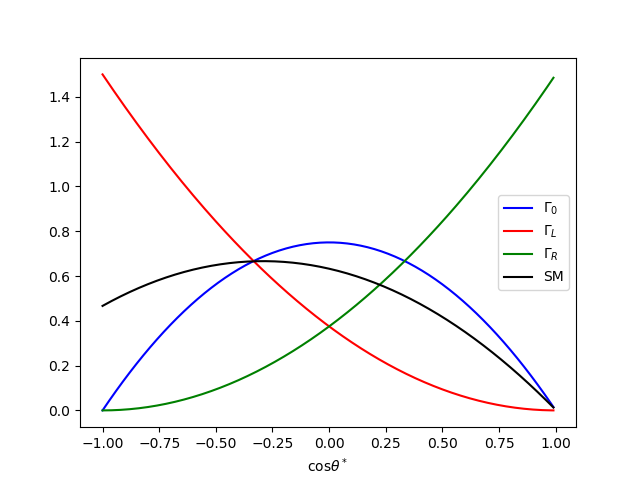
\includegraphics[width=0.7\linewidth]{figures/angular_dist.png}
	\caption{The predicted $\cos \theta^{*}$ angular distribution for helicity
    fractions. The distributions for $F_{0}$, $F_{L}$ and $F_{R}$ are
    normalized, and are given by the blue, red and green line respectively. The
    black line is the sum of the three contributions, but with helicity
    fractions given according to SM predictions.}\label{fig:distributions}
\end{figure}

An approach to obtaining the polarisation states the $W$-bosons, is done by
counting the number of events with a specific $\cos \theta^*$, then use angular
asymmetries, $A_-$, and $A_+$, defined as
\begin{equation}\label{eq:asymmetries}
  A_{\pm}=\frac{N(\cos \theta^* > z)-N(\cos \theta^* < z)}{N(\cos \theta^* > z)+N(\cos \theta^* < z)},
\end{equation}
where $z=\pm(1-2^{2/3})$, is chosen that the asymmetries only has dependence on
$F_0$ and $F_L$ for $A_+$, or $F_0$ and $F_R$ for $A_-$. From
equation~\eqref{eq:asymmetries}, the helicity can be extracted using the
following approach;
\begin{align}
\label{eq:asymmetriesplus}
  A_+ &= \int^1_{z_+} \frac{1}{\Gamma}\dv{\Gamma}{\cos \theta^*} \dd{\cos \theta^{*}} - \int^{z_+}_{-1}
      \frac{1}{\Gamma}\dv{\Gamma}{\cos \theta^*} \dd{\cos \theta^{*}} = 3\beta [F_0 + (1+\beta)F_R],\\
\label{eq:asymmetriesminus}
  A_- &= \int^1_{z_-} \frac{1}{\Gamma}\dv{\Gamma}{\cos \theta^*} \dd{\cos \theta^{*}} - \int^{z_-}_{-1}
      \frac{1}{\Gamma}\dv{\Gamma}{\cos \theta^*} \dd{\cos \theta^{*}} = -3\beta [F_0 + (1+\beta)F_L],
\end{align}
where $\beta = 2^{1/3}-1$. From the
equations~\eqref{eq:asymmetriesplus},~\eqref{eq:asymmetriesminus} and
$F_L+F_0+F_R=1$, the following helicity fractions for the $W$ boson is obtained;
\begin{align}
  F_R&=\frac{1}{1-\beta}+\frac{A_- - \beta A_+}{3\beta (1-\beta^2)},\\
  F_L&=\frac{1}{1-\beta}-\frac{A_+ - \beta A_-}{3\beta (1-\beta^2)},\\
  F_0&=-\frac{1+\beta}{1-\beta}+\frac{A_+ - A_-}{3\beta (1-\beta)}.
\end{align}
The values for angular asymmetries is calculated in SM
NNLO as $A_+=0.537 \pm 0.004$ and
$A_-=-0.841 \pm 0.006$~\cite[24]{CastroNunesFiolhais:1544047}.
%kilde findes på forsøgs artiklen.

\section{Apparatus}
\subsection{LHC}
In the Large Hadron Collider, top quarks are mainly produced through violent
collisions of protons, causing gluon-gluon fusion, which produces top, anti-top
pairs $gg \rightarrow t\bar t$. The data used in this thesis, is from the 2016 run at LHC,
with a centre-of-mass energy of $\sqrt s = 13 \mathrm{TeV}$, which corresponds
to an integrated luminosity of 10 $\mathrm{fb}^{-1}$\cite{oreach2020}. At these
energies, the protons are accelerated close to the speed of light before their
collisions in the ATLAS detector.\\

This process starts, when protons are generated from an ion source in the linear
accelerator, LINAC2, then gets injected into the LHC, through a series of
smaller synchrotron accelerators, as Figure~\ref{fig:lhc} illustrates; Proton
Synchrotron Booster (PSB), Proton Synchrotron (PS) and Super Proton Syncrotron
(SPS)~\cite[135]{Evans_2008}. The LHC receives bunches from SPS, containing many
protons in each bunch, effectively increasing the cross-sectional area for
collisions to occur. The LHC was built to be the largest particle accelerator in the
world, which has allowed it to reach higher energies than other accelerators. At
these energies, more events happen inside the detector, described by the
following equation:
\begin{equation}
  N = \sigma \int L \dd t,
\end{equation}
where $N$ is the number of expected events, $\sigma$ is the cross-sectional area of
the events, and $\int L \dd t$ is the integrated luminosity.

\begin{figure}[H]
	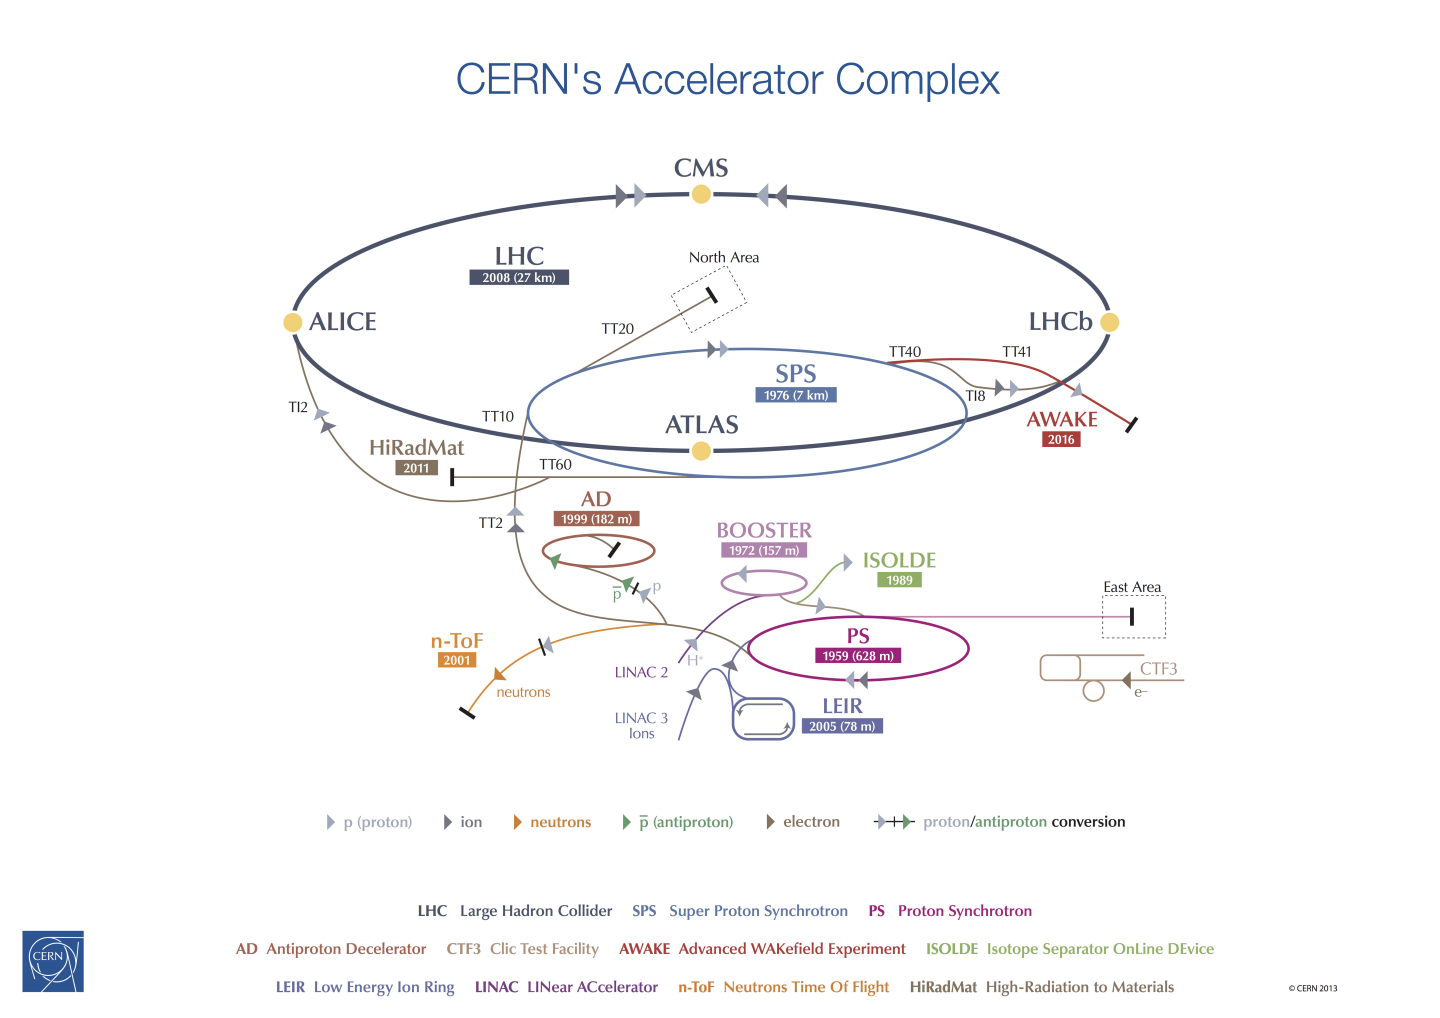
\includegraphics[width=\linewidth]{figures/cern.jpg}
	\caption{The scheme shows the accelerator and detector layout at
    CERN~\cite{Haffner:1621894}.}\label{fig:lhc}
\end{figure}
%evt fjerner jeg labels i bunden senere.

% Cern Thesis af Satoshi Hasegawa
%http://opendata.atlas.cern/release/2020/documentation/datasets/files.html

\subsection{ATLAS}
% https://atlas.web.cern.ch/Atlas/TP/NEW/HTML/tp9new/tp9.html
% https://atlas.cern/discover/detector
% https://en.wikipedia.org/wiki/ATLAS_experiment#ATLAS_detector
% Gamle hjemmeside: https://web.archive.org/web/20110614103207/http://atlas.ch/detector.html

% potential figure https://commons.wikimedia.org/wiki/File:ATLAS_Drawing.jpg


In short, the ATLAS detector consists of multiple components. The first part is
the Inner Detector it tracks charged particles; it is very light to minimize
interaction with the particles. The next part of the detector is the
calorimeters, they stop all particles but muons and neutrinos and measure their
energy. The last part is the muon chambers which serves as extra identification
of muons. The subcomponents are described in more detail below.

\begin{figure}[H]
	\centering
	\includegraphics[scale=0.1]{figures/atlas.jpg}
	\caption{A computer generated image of the ATLAS detector~\cite{detector}}\label{fig:detector}
\end{figure}

\subsubsection{The Inner Detector}
The purpose of this component is to measure charge and momentum, including its
direction, of the detected particle. It consists of three subcomponents.
\paragraph{Pixel Detector}
% https://iopscience.iop.org/article/10.1088/1748-0221/3/07/P07007
The pixel detector consists of approximately 92 million electronic channels.
It's used for identification and reconstruction of secondary vertices from decay
of particles containing a b-quark or for b-tagging jets. The pixel detector
covers pseudorapidity range $|\eta| < 2.5 $
% Og mange flere kriterier relevant?

\paragraph{Semiconductor Tracker}
%https://cds.cern.ch/record/1019885/files/indet-pub-2007-007.pdf
The Semiconductor tracker is a silicon microstrip tracker consisting of 4088
two-sided modules and over 6 million readout strips. These readout strips are
distributed every $80\mathrm{\mu m}$ which allows recording of the position of
charged particles to an accuracy of $17\mathrm{\mu m}$

\paragraph{Transition Radiation Tracker.}
The transition radiation tracker is a drift tube tracker which consists of a
straw with 4mm diameter and 0.03mm diameter tungsten wire, coated with 0.5--0.7mm
gold. The tube is filled with a mixture of Xe, $\mathrm{CO_2}$ and
$\mathrm{O_2}$ gasses. When charged particles travel through the tube the gas
gets ionized, which frees electrons from the gas that move to the gold wire. The
negative charge measured on the wire can be used to distinguish which charged
particle ionized the gas~\cite{ATLAS-ID}. The Inner detector and its
subcomponents can be seen in Figure~\ref{fig:detector}.


\subsubsection{Calorimeter}
% TODO
% Maybe Expand ECal
Calorimeters measure the energy of particles by absorbing them. There are two
types of calorimeters used in the ATLAS detector; the Electromagnetic
Calorimeter (ECal) and Hadronic Calorimeter (HCal). ECal measures electrons and photons.


The HCal consist of scintillator plates that radiates light when exposed to a
charged particle. When a hadron passes through a scintillator plate it produces
a shower of particles which then makes the scintillator radiate light. The
intensity of the radiated light can then be analysed to measure the energy of
the hadron. The calorimeters can be seen in Figure~\ref{fig:detector}.\cite{detector-vid}


\subsubsection{Muon Spectrometer}
% https://atlas.web.cern.ch/Atlas/TP/NEW/HTML/tp9new/node11.html#SECTION00434000000000000000
% https://atlas.cern/discover/detector/muon-spectrometer
% https://en.wikipedia.org/wiki/ATLAS_experiment#Muon_Spectrometer

The muon spectrometer is on the outer part of the ATLAS detector it operates in
the pseudorapidity range $|\eta| < 2.7$. The muon spectrometer is located on the
outside of the detector as other particles will have been stopped earlier in the
calorimeters. The muon spectrometer consists of tubes, much like the transition
radiation tracker, that contains a wire which is surrounded by a gas. When muons
go through these tubes they interact with the gas and leave behind a trail of
ions and electrons which drift towards the wire in the centre. By detecting the
starting point of these trails and measuring the time it takes to reach the
wire, it is possible to determine the position of the muon. The Muon
Spectrometer can be seen in Figure~\ref{fig:detector}.\cite{ATLAS-Muon}


\subsubsection{Data Collection}
The detector generates 60 terabytes of data per second from the 1.7 billion
collisions taking place in the detector in that time frame. However, only a
small sample of the raw data is necessary to reconstruct the collisions. To make
the data more manageable ATLAS uses a two-level trigger system to only save the
most important data. The first part of the trigger system is hardware based, and
can at most save 100 000 events per second, which then gets passed on to the
software based High-Level Trigger. After passing through both triggers, only
approximately 1000 events out of the initial 1.7 billion are saved for later
analysis.\cite{ATLAS-trig}


\subsection{Monte Carlo Simulation}
Monte Carlo (MC) simulation is used in modelling the signal and background
processes expected at the LHC.\@ For the 13 TeV Atlas Open Data used in this
thesis, this process follows four steps; starting with an event generation which
uses an MC generator to mimic the initial pp collision. In the second step,
detector simulation, the geometry of the ATLAS detector and its material
properties gets simulated. The digitization step, follows the previous step by
simulating the responding signals in read-out data, written in a format
compatible with real output of the detector. Finally, these data can be used to
reconstruct the collisions, particle trajectories and subsequent
products.\\

In The 13 TeV ATLAS Open Data set, there are several SM processes which are
modelled using MC simulations. For the purpose of this report, the MC
simulations on top-quark-pair production was used alongside real data taken from
the detector, to compare theory with real data~\cite{mcopenatlas}.

\subsubsection{B-tagging}
To study the $Wtb$ structure, a mechanism to identify the $b$-jets from the
other detected jets is required. First the jets are detected, $b$-hadrons,
$c$-hadrons or light-flavour jets, then their trajectories (tracks) are
reconstructed in the inner detector. Once a jet has been found, the jets
containing b-hadrons are then identified by a combination of three distinct
algorithms. Hadrons containing $b$-quarks have a long enough lifetime to fly a
measurable distance before it decays, and can be exploited to built
lifetime-based tagging algorithms. The impact parameter based algorithm, IP3D,
uses transverse and longitudinal impact parameter significances of each track
within a jet, the SV reconstructs the secondary vertex within the jet and decay
chain multi-vertex algorithm (JetFitter) reconstructs the full b-hadron
decay chain.\\

To better discriminate between jets, a Boosted Decision Tree (BDT) algorithm
called MV2c10, which uses the Root Toolkit for Multivariate Data Analysis
(TMVA), is used to make cuts that discards most of the background components,
the $c$- and light-flavoured jets. For this report, a $b$-jet efficiency rate of
70\% is used, which corresponds to a BDT cut value of 0.8244. This efficiency
rate originates from samples of simulated $t\bar t$ events with a $c$- and
light-jet rejection factor of nearly 400\cite{ATL-PHYS-PUB-2016-012}. At these
cuts, most of the $c$-jets and light-flavoured jets gets rejected, while still
maintaining most of the $b$-jet data.


\section{Data Analysis}
Primarily the ROOT framework was used to process the data from both Delphes and
ATLAS, including detector data and Monte Carlo simulation data. ROOT is a
framework used for storing and processing data in high energy physics. ROOT is
written primarily in the programming language C++, keeping high performance in
mind, such that many gigabytes, if not terabytes or beyond, can be processed in
a reasonable amount of time. Data in ROOT files are stored in a tree format, the
file-format itself being a highly compressed binary file.\cite{root}

\subsection{Results}\label{sec:results}
In order to identify the top-quark-pair production, as seen in
figure~\ref{fig:feynmandiagram}, several cuts in the data were implemented. The
criteria are as follows~\cite{oreach2020}.
\begin{itemize}
  \item Only one electron or muon in the final state with $p_{T} > 30 \mathrm{GeV}$
  \begin{itemize}
    \item Electrons are required to have $|\eta| < 2.47$ aside from $1.37 < |\eta| < 1.52$
    \item Muons are limited by $|\eta| < 2.50$
  \end{itemize}
  \item Missing transverse momentum $E_{T}^{miss} > 30 \mathrm{GeV}$
  \item Transverse mass of the W-boson $M_{T}^{W} > 30 \mathrm{GeV}$
  \item At least four jets with $p_{T} > 30 \mathrm{GeV}$ and $|\eta| < 2.5$, with
        exactly two of these being b-tagged
\end{itemize}

%%%ROOT defines the function \texttt{SetPtEtaPhiE}, which is used in accordance to
%%%Section~\ref{sec:momentum} as seen in equation~\eqref{eq:TLorentz}.
%%%% The function, which ROOT uses to construct the Lorentz vector,
%%%% \texttt{SetPtEtaPhiE}, is defined as such,
%%%\begin{equation} \label{eq:TLorentz}
%%%p({\vb p_t}, \eta, \phi, E) =
%%%\begin{pmatrix}
%%%|{\vb p_t}| \cos(\phi)\\ |{\vb p_t}|\sin(\phi)\\ |{\vb p_t}| \sinh(\eta)\\ E
%%%\end{pmatrix}
%%%\end{equation}
%%%%To calculate the
%%%%transverse energy we are using the builtin ROOT \texttt{TLorentzVector} member
%%%%function \texttt{Et()}. That function is effectively defined as
%%%%\begin{equation}
%%%% {{{\it p\_t}\,\sqrt{{\it p\_y}^2+{\it p\_x}^2}}\over{\sqrt{ {\it p\_z}^2+{\it p\_y}^2+{\it p\_x}^2}}}
%%%%E_t = p_t \frac{\sqrt{p_y^2+p_x^2}}{\sqrt{p_z^2+p_y^2+p_x^2}}
%%%%\end{equation}

Only a single lepton should be present in the events, after the identification
of top-quark pair production. This allows the first lepton in the event to
be used as the leading lepton. Due to the nature of the decay, described in
Section~\ref{sec:coupling}, the tagged lepton can be either an electron or a
muon. This information is used in the construction of the Lorentz vector for the
lepton, from which the transverse momentum is plotted in Figure~\ref{fig:leppt}.\\
% Wait, er det her ikke det samme da M er tæt på nul? Det er måske derfor de
% splitter electron muon. det kan være vi bare skal plotte noget andet eller vi
% kan jo selvfølgelig også bare gøre det samme som de gør ved at splitte
% electron/muon. Vi kan endda også bare plotte histogrammet med partikel id for
% at vise hvor mange af hver der er



\begin{figure*}[t!]
  \centering
  \begin{subfigure}[t]{0.47\textwidth}
    \centering
    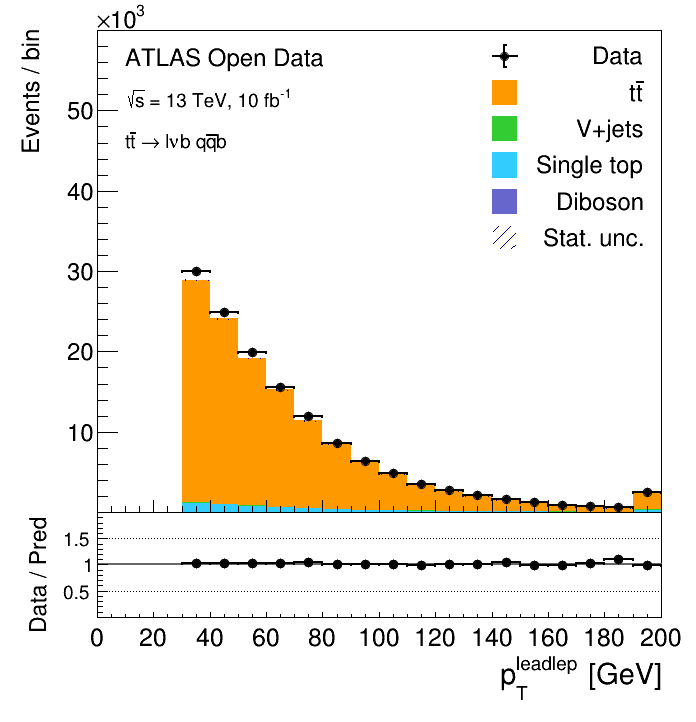
\includegraphics[width=1.0\textwidth]{figures/hist_leadleptpt}
    \caption{\label{fig:leppt}Lead lepton transverse momentum for both
      single-electron and single-muon channel.}
  \end{subfigure}%
  \hfill{}
  \begin{subfigure}[t]{0.47\textwidth}
    \centering
    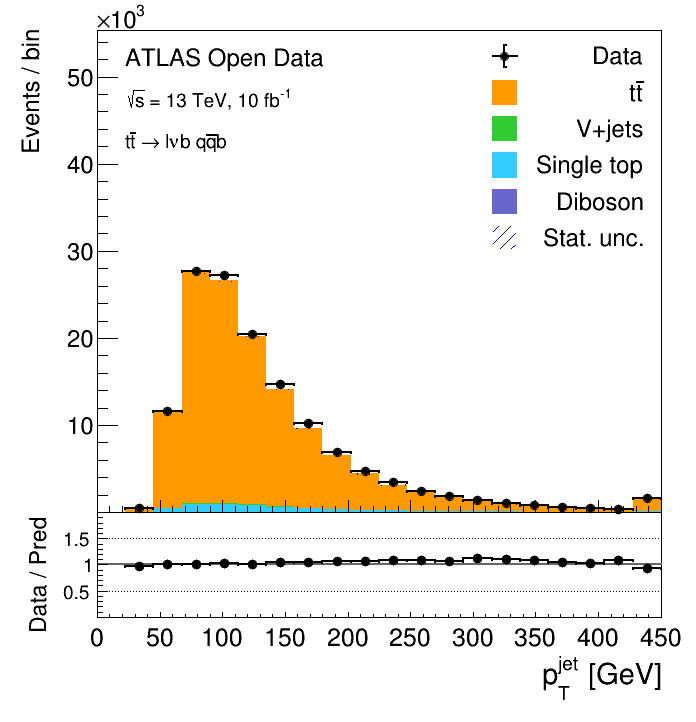
\includegraphics[width=1.0\textwidth]{figures/hist_leadjet_pt}
    \caption{\label{fig:jetpt}Lead jet transverse momentum for both
      single-electron and single-muon channel.}
  \end{subfigure}
  \caption{}
\end{figure*}

In the ATLAS Open Data, the reconstruction of the tracks, and calculation of the
transverse momentum of jets, is already given. The jets in the event are
ordered, which provides information about the leading jet simply by accessing
the first one. Good jets are decided on the requirements given in
Section~\ref{sec:results}, and the momentum plotted in
Figure~\ref{fig:jetpt}. \\% also a requirement on pseudorapidity
% of the jets to be less than 2.5, however this should probably be mentioned in
% the criteria

The missing transverse energy, $E_T^{miss}$, is also given, calculated by
consideration of momentum conservation, in accordance with what is described in
Section~\ref{sec:transmomentum}. The missing transverse energy is then plotted
if the given event satisfies all the criteria given in
Section~\ref{sec:results}. The energy was plotted in the appropriate units in
Figure~\ref{fig:etmiss}.\\

\begin{figure*}[t!]
    \centering
    \begin{subfigure}[t]{0.47\textwidth}
      \centering
      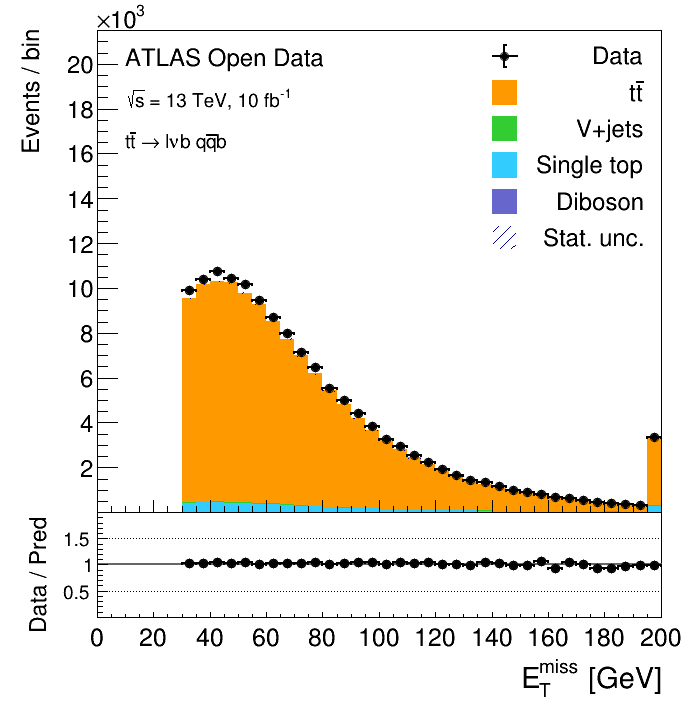
\includegraphics[width=1.0\textwidth]{figures/hist_etmiss}
      \caption{\label{fig:etmiss}Missing transverse energy for both
        single-electron and single-muon channel.}
    \end{subfigure}%
      \hfill{}
    \begin{subfigure}[t]{0.47\textwidth}
      \centering
      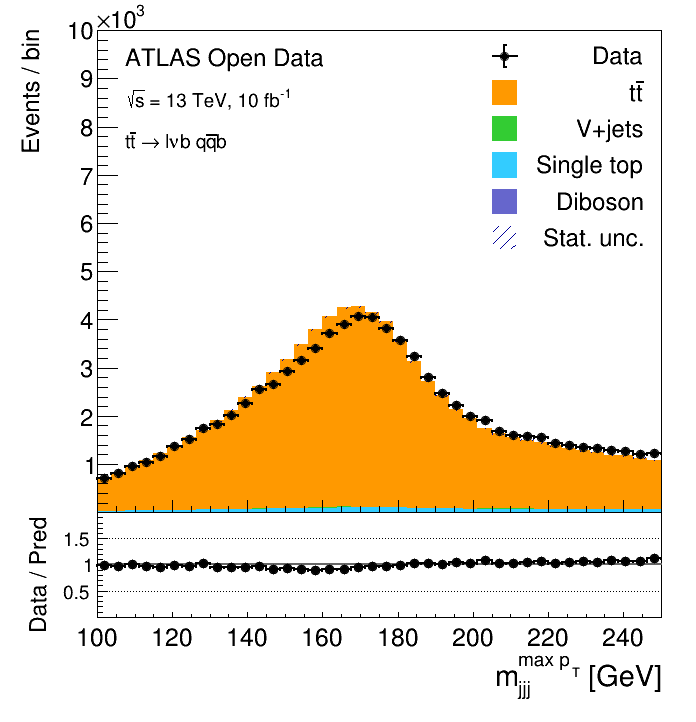
\includegraphics[width=1.0\textwidth]{figures/hist_Topmass}
      \caption{\label{fig:topmass}Top quark mass from the ATLAS data.}
    \end{subfigure}
    \caption{}
\end{figure*}

% maybe explain why maxing Pt gives the lower three jets but seems a bit
% obvious: if the b-jet in the upper part was in the combination it would
% subtract from the transverse momentum because it was produced from the top
% quark which has opposite momentum from the anti top quark.
The top quark mass can be calculated by finding the combination of three jets,
of which one is a $b$-jet, with the highest transverse momentum, and taking the
mass of the whole three jet system. This is a utilization of the hypothesis,
that these three jets are the ones produced by the $\overline{t}$-quark in the
lower part of the Feynman diagram seen in Figure~\ref{fig:feynmandiagram}. While
this hypothesis would most likely hold for most events, it is unlikely to hold
for all.
% possible explanation why it works here (see comment above)
Once the top quark mass is found it can be plotted, as seen in
Figure~\ref{fig:topmass}. The peak of this histogram should then be compared to
the value from the standard model, which is $172.76 \pm 0.30$ GeV\cite{pdg}.

\subsection{$\cos \theta^{*}$ reconstruction}
Reconstruction of $\cos \theta^{*}$ from the data given in the Lorentz four-vectors, was
accomplished by equation~\eqref{eq:costheta}. Since only two $b$-jets is tagged,
the $b$-jet associated with the leptonic decay was decided by the method of
exclusion, once the $b$-jet associated with the other jets was identified. The
reconstructed $\cos \theta^{*}$ is plotted in Figure~\ref{fig:costhetaatlas} below.
\begin{figure}[H]
  \centering
  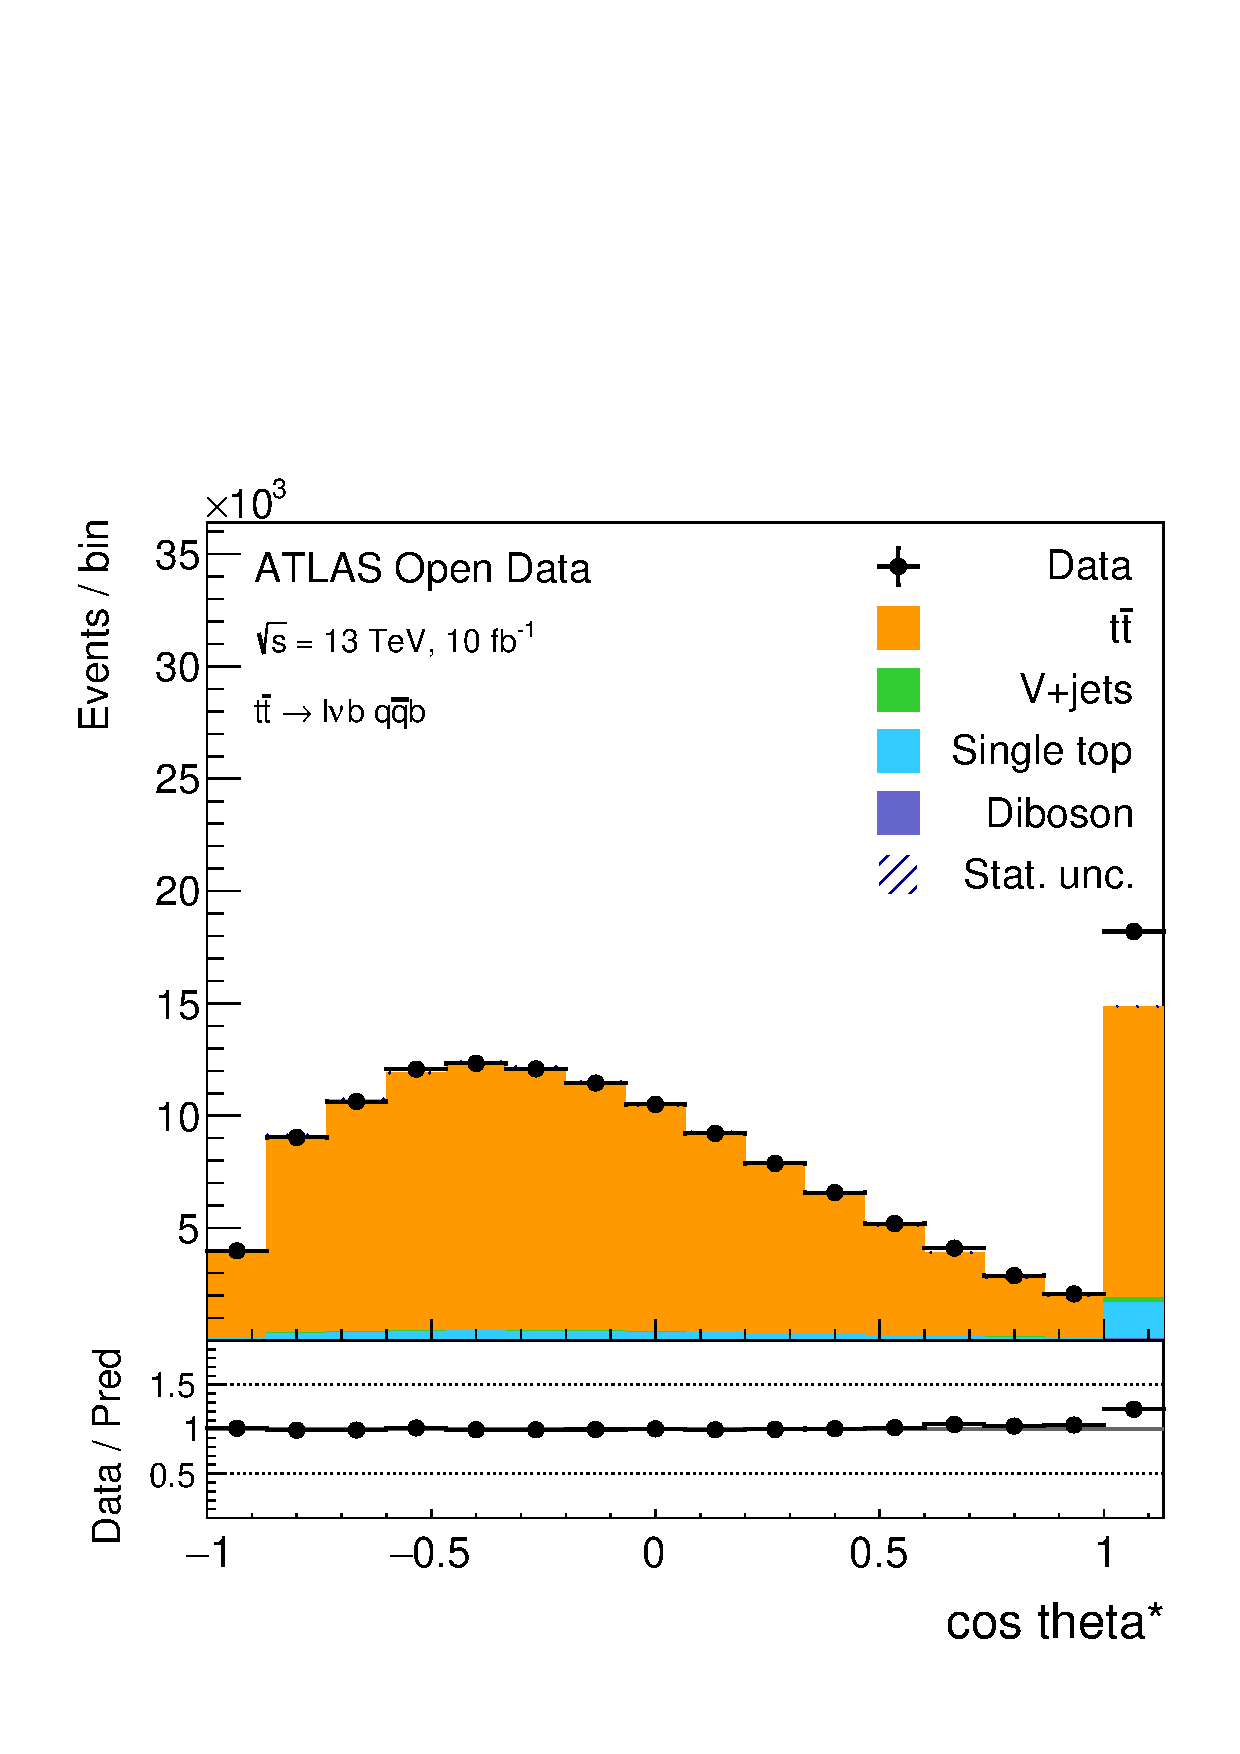
\includegraphics[width=0.6\textwidth]{figures/hist_costheta_overflow}
  \caption{\label{fig:costhetaatlas}Reconstructed $\cos \theta^{*}$ from ATLAS data. Overflow is in the last bin.}
\end{figure}

\subsection{Angular Asymmetries}
% TODO:
% Kilde til konstant selection ratio?
For measurements of angular asymmetries $A_{\pm}$ from
equation~\eqref{eq:asymmetries}, the $\cos\theta^{*}$ distribution was split into
three non-uniform bins with events above and below
$z_{\pm} = \pm(1-2^{\frac{2}{3}})$ given by; $N_1 = N(\cos \theta^{*}<z_-)$,
$N_3 = N(\cos \theta^{*}>z_+)$ and $N_2$ being the remaining events. The true
$\cos\theta^*$ distribution has a constant selection ratio over all angles $\cos\theta^*$,
and the simulated $\cos\theta^*$ distribution does
not.\\

Therefore, correction factors $c_1$ and $c_3$ for bin $N_1$ and $N_3$
respectively are calculated for the simulated $\cos\theta^*$ distribution to match
the Standard Model values of $A_{\pm}$, and thereby giving a constant selection ratio of $\cos\theta^*$.
\begin{align}
	A_{+}^{SM} &= \frac{(c_3N_3 + N_2) - c_1N_1}{c_1N_1 + N_2 + c_3N_3} \\
	A_{-}^{SM} &= \frac{c_3N_3 - (c_1N_1 + N_2)}{c_1N_1 + N_2 + c_3N_3}
\end{align}
Solving for the correction factors the following values are obtained.
\begin{align} \label{eq:correction}
	c_1 &= \frac{N_2(1-A_{+}^{SM})}{N_1(A_{+}^{SM} -A_{-}^{SM})} = \num{1.15 +- 0.01}  \\
	c_3 &= \frac{N_2(A_{-}^{SM}+1)}{N_3(A_{+}^{SM}-A_{-}^{SM})} = \num{1.10 +- 0.05}
\end{align}
For measurements of angular asymmetries, correction factors and helicity fractions
the error was found using first order error propagation.
%\begin{align}
%\sigma_{c_1} = \sqrt{\left(\pdv{c_1}{N_1}\right)^2\sigma_{N_1}^2 + %\left(\pdv{c_1}{N_2}\right)^2\sigma_{N_2}^2 + %\left(\pdv{c_1}{A_+}\right)^2\sigma_{A_+}^2 + %\left(\pdv{c_1}{A_-}\right)^2\sigma_{A_-}^2}
%\end{align}
\begin{align}
	\sigma_{f} = \sqrt{\sum_{i}\left(\pdv{f}{x_i}\right)^2\sigma_{x_i}^2}
\end{align}
Due to limitations of the Open Atlas Data~\cite{oreach2020}, only statistical
uncertainties were considered, leaving the possibility of larger systematic
uncertainties.\\

The correction factors obtained from simulation is then applied to the
$\cos\theta^{*}$ distribution from the ATLAS data, leading to the angular asymmetries
$A_- = -0.831 \pm 0.006$ and $A_+ = 0.542 \pm 0.005$, resulting in the helicity
fractions $F_0=0.678 \pm 0.015$, $F_L=0.308 \pm 0.008$ and $F_R=0.014 \pm 0.009$.

\subsection{Template Method}
As an alternative to finding the helicity fractions using angular asymmetries,
the Template Method was used by generating a different data set for each of the
possible polarisation states. These simulations weren't available through the
ATLAS Open Data, and without the time and access to a preferred full simulation,
a fast simulation, which could emulate the response of the detector,
was employed.\\

Pythia was used to generate $t\bar t$-events, which produced four momentum
vectors for all the final state particles in the $p-p$ collisions. This gave
three files containing left, longitudinal and right-handed polarisations of the
W-boson separately. These files were then run through Delphes, which emulates
the ATLAS detector response and uses that to reconstruct the particles. Cuts
were applied in ROOT matching the event selection criteria defined in
Section~\ref{sec:results} to filter out background data. The normalised
templates were then combined and fitted to the normalised $\cos \theta^{*}$
distribution from the ATLAS detector in a linear combination, giving the three
helicity fractions $F_L$, $F_R$ and $F_0$. The fitted coefficients are the
contribution of the corresponding state to the primary data.\\

Because Pythia doesn't give the spin orientations of the $W$-boson, for each
event, as it describes the SM, giving very few events produced at
$\cos \theta^{*} \rightarrow 1$. This complication was resolved, using a workaround, where the
$W$ decay to lepton+neutrino was found. For half of the events, the identity
lepton and neutrino was switched, so the neutrino travelled in the direction
that the lepton did, and vice versa. $\cos \theta^{*}$ was calculated for each event
using equation~\ref{eq:costheta}. Importance sampling was used to match the
theoretical distribution, generating the three distributions given in
Figure~\ref{fig:delphesdist}. The size of these files, limited the number of
generated events to 20,000 for each of the three distribution, resulting in even
fewer remaining events after cuts.

% http://opendata.atlas.cern/release/2020/documentation/physics/SL3.html

\subsection{Delphes data}
Before the criteria from Section~\ref{sec:results} were applied to the Delphes
data, a sanity check was performed on the generated truth data, to assess
whether it matches with the theoretical analytical function plotted in
Figure~\ref{fig:distributions}. The plot for each of the three polarisations is
displayed in Figure~\ref{fig:delphesdist}. The fitting, in this case, is just a
scaling factor, as the generated distributions are not normalised.
\begin{figure*}[t!]
    \centering
    \begin{subfigure}[t]{0.5\textwidth}
        \centering
        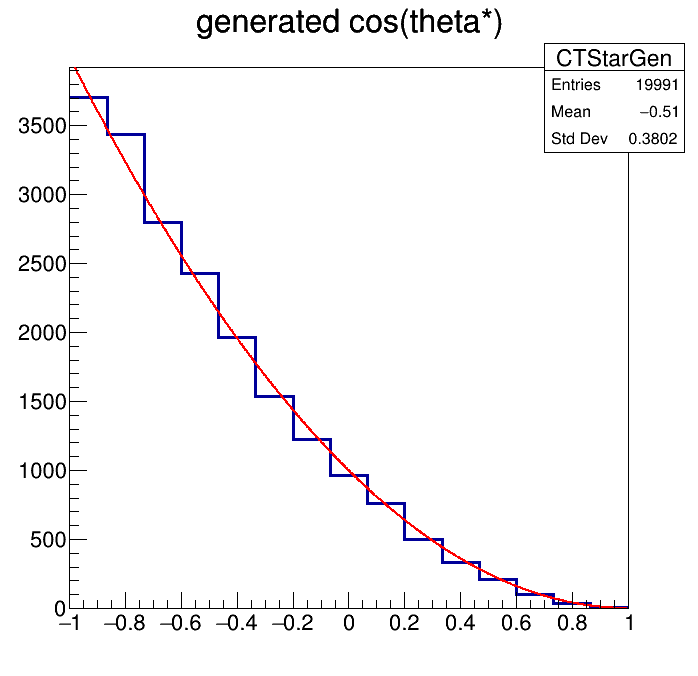
\includegraphics[width=1.0\textwidth]{figures/delphes_genL}
        \caption{$F_L$ generated distribution.}
    \end{subfigure}%
    \begin{subfigure}[t]{0.5\textwidth}
        \centering
        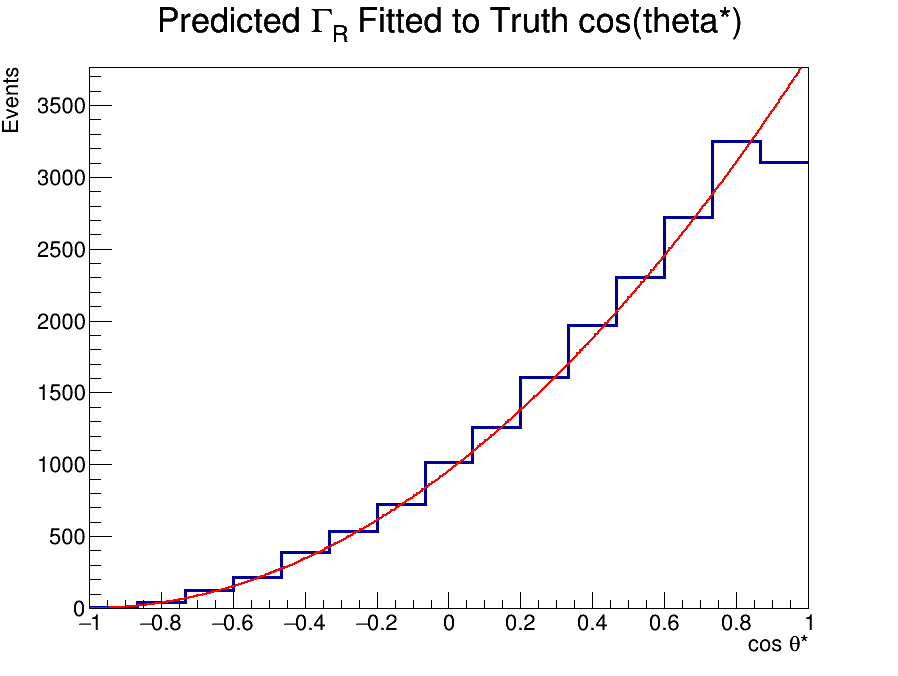
\includegraphics[width=1.0\textwidth]{figures/delphes_genR}
        \caption{$F_R$ generated distribution.}
      \end{subfigure}
    \begin{subfigure}[t]{0.5\textwidth}
        \centering
        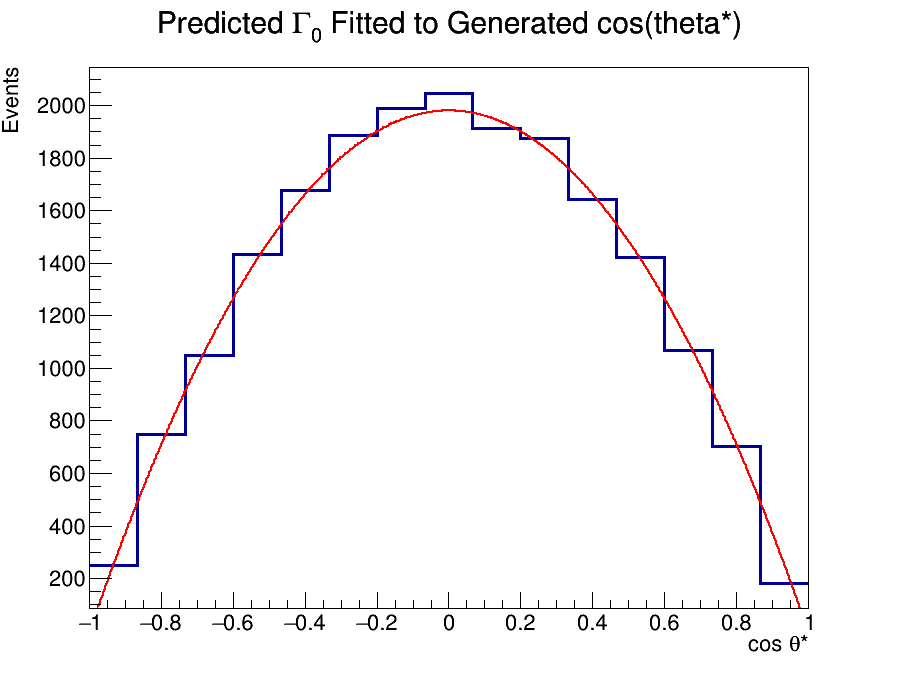
\includegraphics[width=1.0\textwidth]{figures/delphes_gen0}
        \caption{$F_0$ generated distribution.}
    \end{subfigure}
    \caption{The figures shows the truth values of the generated $F_L$, $F_R$ and
      $F_0$ distributions, with a sample of 20000 events, using Delphes fast
      simulations to generate.}\label{fig:delphesdist}
\end{figure*}

Using the generated distributions and the criteria described in
Section~\ref{sec:results}, it is now possible to generate an efficiency
distribution as a function of $\cos \theta^*$ for the specified criteria.

\begin{figure}[H]
  \centering
  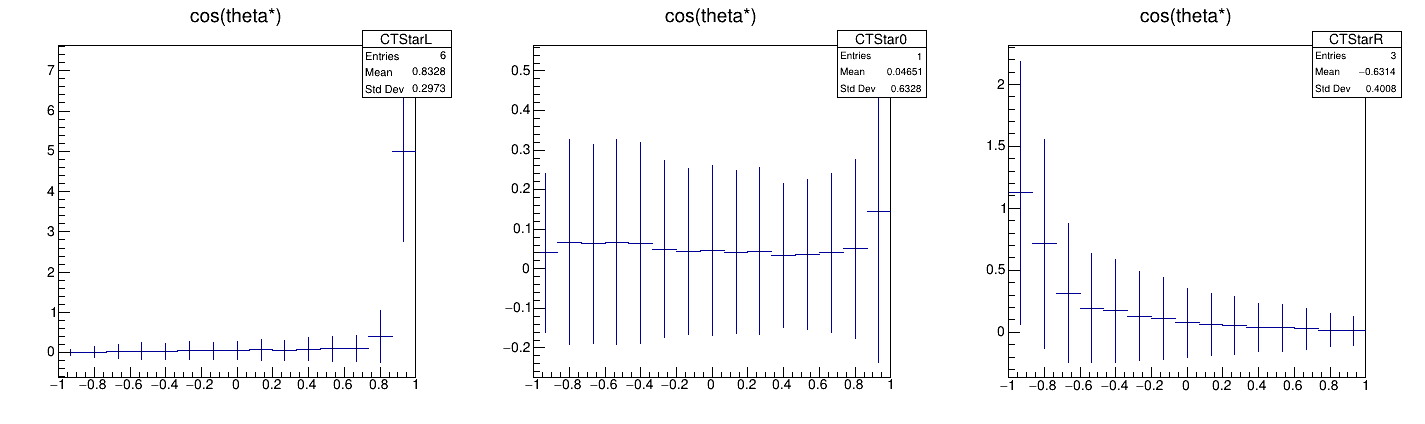
\includegraphics[width=0.7\textwidth]{figures/efficiency}
  \caption{\label{fig:efficiency}These efficiencies are obtained by dividing the
    the sum of the three histograms of the generated values for the samples that
    remained after the cuts by the sum of the three histograms of all the
    generated values.}
\end{figure}

To reconstruct the helicity distributions which would be found from
measurements, the criteria performed on the ATLAS data, from
Section~\ref{sec:results}, were matched on the Delphes data, to isolate the
equivalent usable data, gotten from the ATLAS detector. The
Figure~\ref{fig:redelphesdist} shows the three helicity distributions after the
cuts.
\begin{figure*}[t!]
  \centering
  \begin{subfigure}[t]{0.47\textwidth}
    \centering
    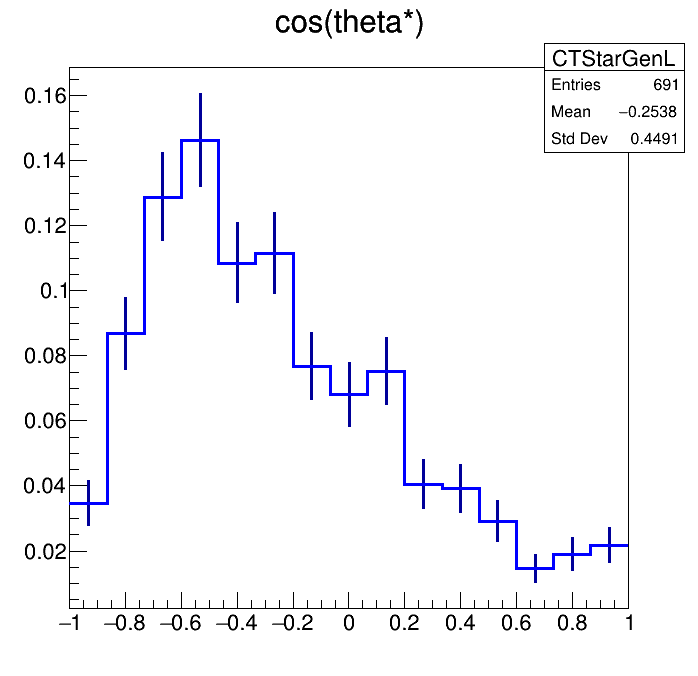
\includegraphics[width=1.2\textwidth]{figures/delphes_ctstarL}
    \caption{$F_L$ normalised reconstructed distribution with 691 remaining events.}
  \end{subfigure}\hfill{}%
  \begin{subfigure}[t]{0.47\textwidth}
    \centering
    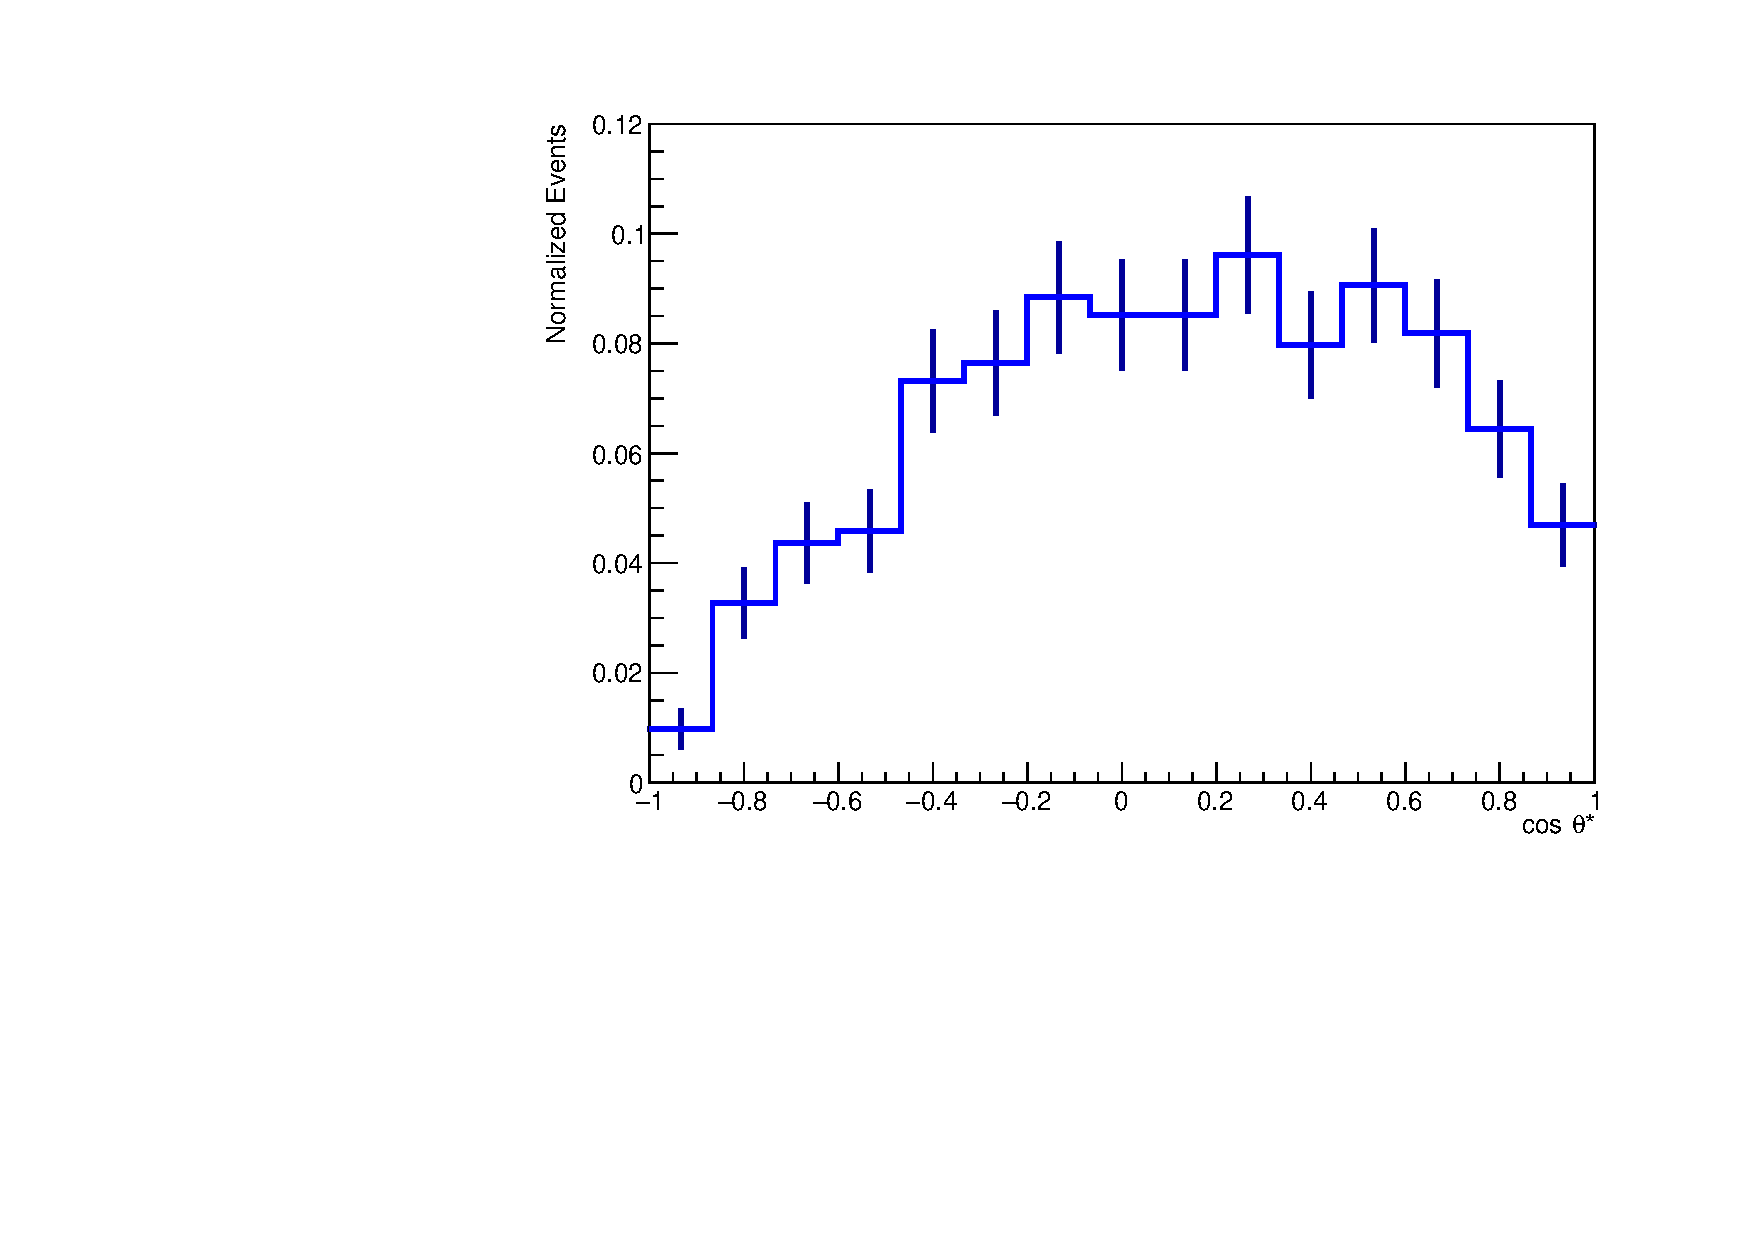
\includegraphics[width=1.2\textwidth]{figures/delphes_ctstarR}
    \caption{$F_R$ normalised reconstructed distribution with 916 remaining events.}
  \end{subfigure}
  \begin{subfigure}[t]{0.5\textwidth}
    \centering
    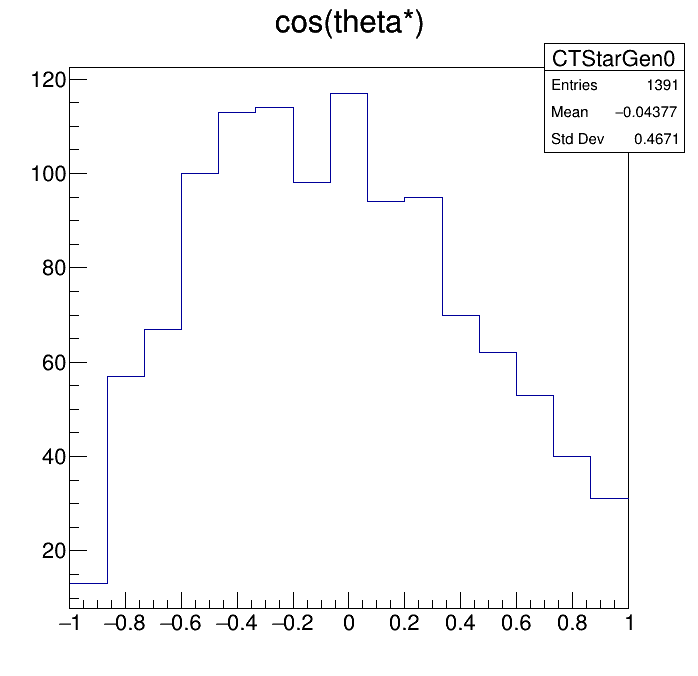
\includegraphics[width=1.1\textwidth]{figures/delphes_ctstar0}
    \caption{$F_0$ normalised reconstructed distribution with 981 remaining events.}
  \end{subfigure}
  \caption{The figures shows the normalised reconstructed Delphes $\cos \theta^*$ from the
    generated $F_L$, $F_R$ and $F_0$ distributions after the same cuts were made
    as the ones made on the Open ATLAS data.}\label{fig:redelphesdist}
\end{figure*}


To get an idea of how the shape of the $\cos \theta^*$ values change as they are
reconstructed, the true values are plotted versus the reconstructed values in
Figure~\ref{fig:2dhist}. The diagonal line in this plot is the expectation and
indicates no change in $\cos \theta^*$ during reconstruction. Anything below this
line is a shift towards lower values and anything above it is a shift towards
higher values. In the plot there is clearly a higher number of events below the
diagonal line than above it, which, as was just discussed, means a general shift
towards lower $\cos \theta^*$ values.
\begin{figure}[H]
  \centering
  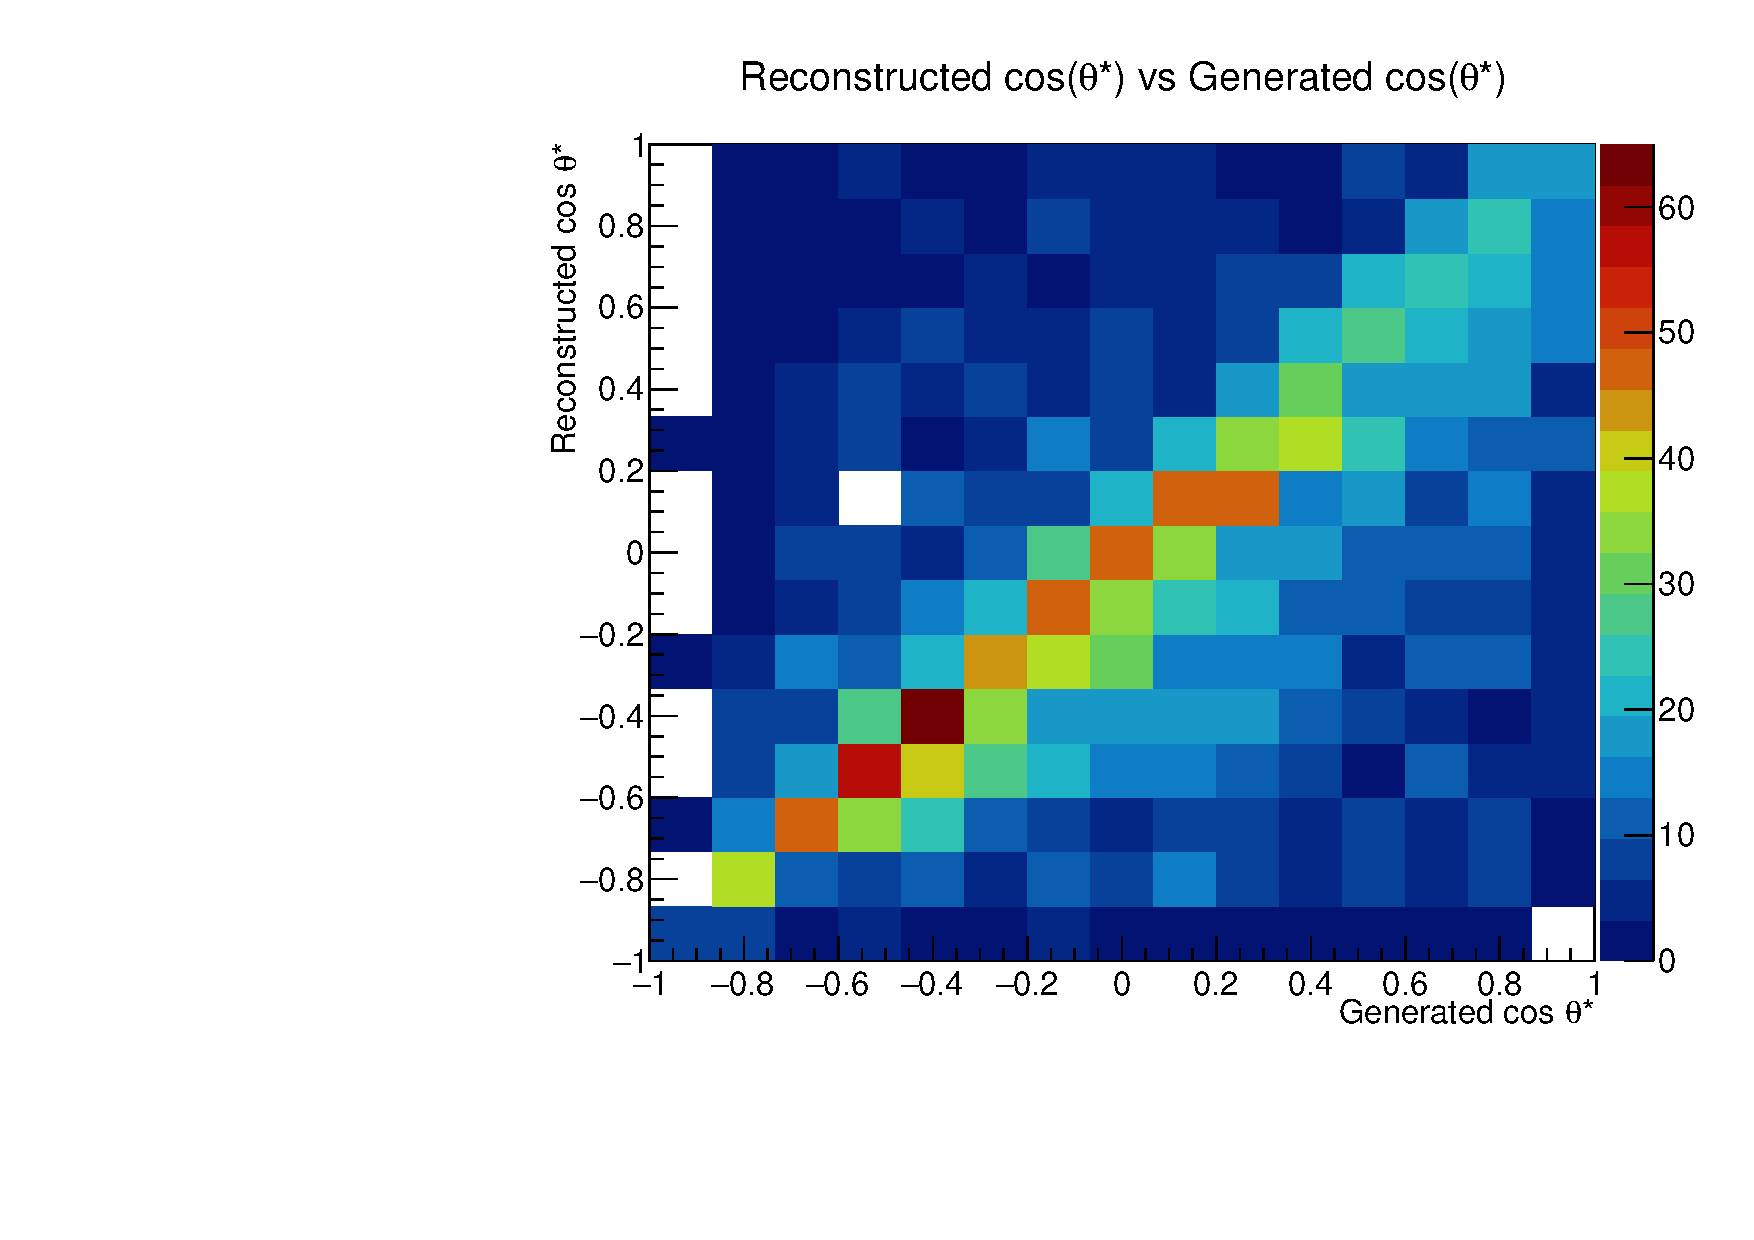
\includegraphics[width=0.6\linewidth]{figures/2dhist}
  \caption{\label{fig:2dhist} On the $x$-axis are the generated true $\cos \theta^*$ values for
    the events which remained after the cuts, and on the $y$-axis are the
    reconstructed $\cos \theta^*$ for the same events.}
  % 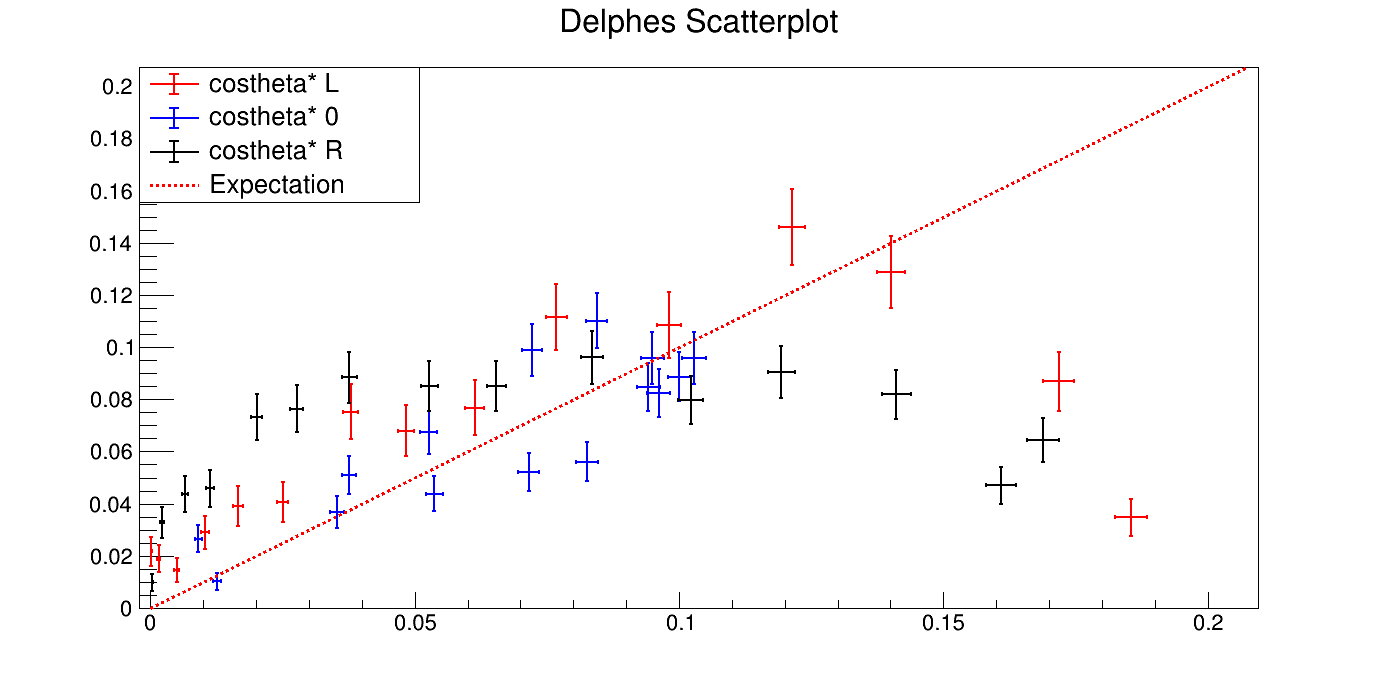
\includegraphics[width=\linewidth]{figures/scatterplot}
  %\caption{\label{fig:scatterplot}Every point represents a bin. The $x$-value is
  %  the normalized truth value, and the $y$-value is the normalized value after
  %  the cuts in the data have been made. From this it is possible to see how the
  %  shape of the histograms change after the cuts. The extremes are cut off and
  %  histogram for $h=0$ is shifted to a side which can be seen by the symmetric
  %  shape around the expectation line.}
\end{figure}


% maybe move or remove this?
\begin{figure}[ht]
  \centering
  \begin{tabular}[H]{|c|c|c|c|}
    \hline
    $h=-1$    & $h=0$     & $h=+1$    & Sum       \\\hline
    $3.457\%$ & $4.932\%$ & $4.754\%$ & $4.375\%$ \\\hline
  \end{tabular}
  \caption{\label{fig:delphesefficiency}Efficiency table calculated by dividing
    the reconstructed $\cos \theta^*$ histogram entry count by its corresponding truth value histogram entry
    count.}
\end{figure}


\subsection{Fitting to atlas data}
The histograms shown in Figure~\ref{fig:redelphesdist}, is fitted by a linear
combination of parameters, to the histogram containing the ATLAS data.
Figure~\ref{fig:delphesfit} displays the fitted data, and below is listed the
obtained parameters, corresponding to the helicity fractions, alongside the
error associated with the iterative approach to the fit.

\begin{figure}[H]
  \centering
  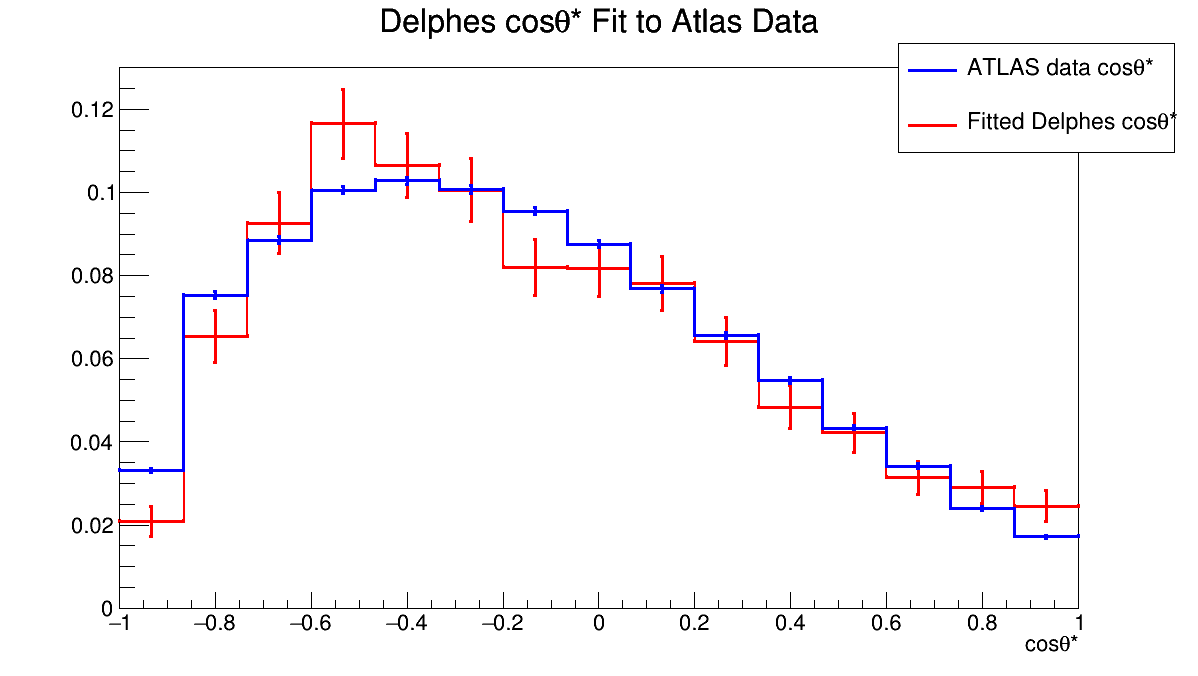
\includegraphics[width=0.9\textwidth]{figures/delphes_fit}
  \caption{\label{fig:delphesfit}Reconstructed Delphes $\cos \theta^{*}$ fitted to
    the $\cos \theta^{*}$ from ATLAS data.}
\end{figure}


% TODO husk at opdatere errors når vi finder ud af det
The fit in Figure~\ref{fig:delphesfit} gave the following helicity fractions,
$F_0^{\mathrm{fit}} = 0.511 \pm 0.017,\ F_L^{\mathrm{fit}} = 0.441 \pm 0.009$,
and $F_R^{\mathrm{fit}} = 0.031 \pm 0.009$, with a $\chi^2 = 1963.72$. The error
here is the numerical error directly from the fit and should be adjusted
to......................
%% \begin{verbatim}
%% FCN=1963.72 FROM MIGRAD  STATUS=CONVERGED  61 CALLS     62 TOTAL
%%        EDM=2.23898e-18    STRATEGY= 1      ERROR MATRIX ACCURATE
%%  PARAMETER  VALUE        ERROR        STEP SIZE   1st DERIVATIVE
%%  F_0        5.11016e-01  1.71117e-02  6.08806e-05  -5.60212e-07
%%  F_L        4.41250e-01  9.31108e-03  6.00363e-05  -6.62772e-07
%%  F_R        3.13704e-02  9.18531e-03  5.33415e-05  -3.72978e-07
%% CHI2 : 1963.72
%% \end{verbatim}


\section{Discussion}
The plots, constructed using the ATLAS data, was presented in the preceding
section. The data given in Figures~\ref{fig:jetpt},~\ref{fig:leppt} and
Figures~\ref{fig:etmiss},~\ref{fig:topmass}, are in good agreement with the
simulated events, with low level of background events. The simulations of the
top mass was completed using a $m_t = 172.5 \mathrm{GeV}$~\cite{oreach2020},
which could account for the small deviation, if the data favours a different
mass.

The 13 TeV Open Datasets did not simulate polarisations of the $W$ boson,
leading to the utilization of Delphes, in getting polarisation distributions to
fit to the reconstructed $\cos \theta^{*}$ data. The greatest source of errors is a
consequence of statistical errors, due to the small number of event samples
surviving the cut on the given Delphes data, where less than 1/20 of the events
survives the cuts from truth to reconstructed. This results in much more
statistic from the ATLAS data, than from the Delphes simulations. The
uncertainties on the helicity fractions only take error associated with the
statistical fluctuations of the Atlas data into consideration, therefore the
uncertainties presented are greatly underestimated.\\ %noget om at forsøge at estimere højere usikkerheder

Figure~\ref{fig:efficiency} illustrates that the efficiency is not flat as a
function of $\cos \theta^{*}$, but has lower efficiency in $\cos \theta^{*} < z_+$. This
possible originates from the criteria on lepton tagging, where it is required
that they appear isolated in the detector. At $\cos \theta^{*} \rightarrow -1$, the $b$ quark
and the lepton are moving in the same direction, making it impossible to detect
the lepton, and erasing the event from the single lepton channel. The 2D plot of
Figure~\ref{fig:2dhist}, further reinforces this assertion, where the shift
below the diagional line, represents the fact that the reconstructed values
diverges more from the truth vlues, at lower $\cos \theta^{*}$, the reconstructed
plot moves towards the left.\\

Since Delphes runs a fast-simulation, it is not designed to be used in parallel
with data taken from advanced detector studies. This analysis could consequently
serve as a test for this approach of combining Delphes simulations with data
taken from ATLAS detector, but the great statistical uncertainty, due to the low
number of simulated events, makes any reasonable conclusion on this approach
impossible. Instead, as a result of time constraints, and the large storage
space required to simulate a sufficient number of Delphes events, information
about the $W$ polarisation was obtained by the method of angular
asymmetries, described in Section~\ref{sec:coupling}.\\

Measurements using angular asymmetries were more accurate with less statistical
errors, due to the fact that the data was taken exclusively from the Open ATLAS
Data, which had a much larger data sample than the Delphes simulations. This
allowed for a more confident evaluation of the $W$ boson's helicity fractions.\\



%Det her skal nok stå et sted i Delphes delen, hvis det skal stå et sted
%While similar cuts was attempted to be implemented on the Delphes'
%truth-information, due to the absence of the b-tagging MV2c10 algorithm in
%Delphes, cuts were made using
%80--85\% efficiency instead~\cite{CMS-PAS-BTV-11-004}.\\




%Forklaring om overflow, ved ikke hvor meget der er relevant.
%The reconstructed $\cos \theta^*$, from the ATLAS data, used in both methods, had
%significant entries in overflow. The theoretical $\cos \theta^*$ was compared to the
%approximation, but no significant differences appeared between the two, refuting
%the possibility that overflow stemmed from the approximation.
%This %ved ikke om vi overhovedet bør nævne det med den sammenligningen.
%overflow was ignored in the fitting process, as only data remaining within the
%physically possible range from -1 to 1, was considered in the analysis. The
%Delphes data for the helicity distributions, had substantially less overflow,
%than data from Open ATLAS, which also motivated the decision to only fit within
%the parameter -1 to 1.

%error propagation, skal nok stå lidt mere om
%For measurements of angular asymmetries, the error was found, using first order
%error propagation on equation~\eqref{eq:asymmetries}.

%Noget om statistical uncertainty, kan måske skrives som en kort kommentar i
%analysen.
%Due to the limitations of the Open Atlas
%Data~\cite{oreach2020}, only statistical uncertainties were considered, leaving
%the possibility of larger systematic uncertainties.

\section{Conclusion}
A measurement of the polarisation of $W$ bosons, from top quark pair events
decay to single lepton channels, was presented using data collected from Open
ATLAS $pp$ collision at $\sqrt s = 13$TeV, corresponding to an integrated
luminosity of 10 fb$^{-1}$. Owed to the reason that the reconstructed $W$
polarisation data from Delphes had a small event sample, resulting in large
statistical uncertainties, nothing instructive could be concluded from those
data. Instead, the helicity fractions obtained from angular asymmetries are
$F_0=0.678 \pm 0.015$, $F_L=0.308 \pm 0.008$ and $F_R=0.014 \pm 0.009$. These
results are in agreement with the NNLO QCD predictions.


\printbibliography

\end{document}
